%%%%%%%%%%%%%%%%%%%%%%%%%%%%%%%%%%%%%%%%
% datoteka diploma-vzorec.tex
%
% vzorčna datoteka za pisanje diplomskega dela v formatu LaTeX
% na UL Fakulteti za računalništvo in informatiko
%
% vkup spravil Gašper Fijavž, december 2010
% 
%
%
% verzija 12. februar 2014 (besedilo teme, seznam kratic, popravki Gašper Fijavž)
% verzija 10. marec 2014 (redakcijski popravki Zoran Bosnić)
% verzija 11. marec 2014 (redakcijski popravki Gašper Fijavž)
% verzija 15. april 2014 (pdf/a 1b compliance, not really - just claiming, Damjan Cvetan, Gašper Fijavž)
% verzija 23. april 2014 (privzeto cc licenca)
% verzija 16. september 2014 (odmiki strain od roba)
% verzija 28. oktober 2014 (odstranil vpisno številko)
% verija 5. februar 2015 (Literatura v kazalu, online literatura)
% verzija 25. september 2015 (angl. naslov v izjavi o avtorstvu)
% verzija 26. februar 2016 (UL izjava o avtorstvu)
% verzija 16. april 2016 (odstranjena izjava o avtorstvu)
% verzija 5. junij 2016 (Franc Solina dodal vrstice, ki jih je označil s svojim imenom)


\documentclass[a4paper, 12p]{book}
%\documentclass[a4paper, 12pt, draft]{book}  Nalogo preverite tudi z opcijo draft, ki vam bo pokazala, katere vrstice so predolge!

\usepackage[utf8x]{inputenc}   % omogoča uporabo slovenskih črk kodiranih v formatu UTF-8
\usepackage[slovene,english]{babel}    % naloži, med drugim, slovenske delilne vzorce
\usepackage[pdftex]{graphicx}  % omogoča vlaganje slik različnih formatov
\usepackage{fancyhdr}          % poskrbi, na primer, za glave strani
\usepackage{amssymb}           % dodatni simboli
\usepackage{amsmath}           % eqref, npr.
%\usepackage{hyperxmp}
\usepackage[hyphens]{url}  % dodal Solina
\usepackage{comment}       % dodal Solina
\usepackage{listings}
\usepackage{float}
\usepackage[active, generate=filename.txt, extract-env={document}]{extract}

\usepackage[pdftex, colorlinks=true,
						citecolor=black, filecolor=black, 
						linkcolor=black, urlcolor=black,
						pagebackref=false, 
						pdfproducer={LaTeX}, pdfcreator={LaTeX}, hidelinks]{hyperref}
						
\usepackage{pgfplots}

\usepackage{color}       % dodal Solina
\usepackage{soul}       % dodal Solina
\lstdefinelanguage{swift}
{
  morekeywords={
    func,if,then,else,for,in,while,do,switch,case,default,where,break,continue,fallthrough,return,
    typealias,struct,class,enum,protocol,var,func,let,get,set,willSet,didSet,inout,init,deinit,extension,
    subscript,prefix,operator,infix,postfix,precedence,associativity,left,right,none,convenience,dynamic,
    final,lazy,mutating,nonmutating,optional,override,required,static,unowned,safe,weak,internal, integer,
    private,public,is,as,self,unsafe,dynamicType,true,false,nil,Type,Protocol, interface, Int, String, Double, Char, Void, print, type, typ, fun, int, const, NULL, bool, null, Any, abstract, _, def, True, False, putInt
  },
  morecomment=[l]{\#}, % l is for line comment
  morecomment=[s]{/*}{*/}, % s is for start and end delimiter
  morestring=[b]" % defines that strings are enclosed in double quotes
}
\RequirePackage{xcolor}
\definecolor{keyword}{HTML}{BA2CA3}
\definecolor{string}{HTML}{D12F1B}
\definecolor{comment}{HTML}{008400}

\lstset{
  language=swift,
  basicstyle=\ttfamily,
  showstringspaces=false, % lets spaces in strings appear as real spaces
  columns=fixed,
  keepspaces=true,
  keywordstyle=\color{keyword},
  stringstyle=\color{string},
  commentstyle=\color{comment},
  breaklines=true,
  tabsize=2
}

%%%%%%%%%%%%%%%%%%%%%%%%%%%%%%%%%%%%%%%%
%	DIPLOMA INFO
%%%%%%%%%%%%%%%%%%%%%%%%%%%%%%%%%%%%%%%%
\newcommand{\ttitle}{Vgradnja objektno usmerjenih gradnikov v programski jezik PINS}
\newcommand{\ttitleEn}{Implementation of object oriented additions to PINS}
\newcommand{\tsubject}{\ttitle}
\newcommand{\tsubjectEn}{\ttitleEn}
\newcommand{\tauthor}{Toni Kocjan Turk}
\newcommand{\tkeywords}{prevajalnik, programski jezik, sintaksa, semantika, Java, Swift, Atheris}
\newcommand{\tkeywordsEn}{compiler, programming language, syntax, semantics, Java, Swift, Atheris}


%%%%%%%%%%%%%%%%%%%%%%%%%%%%%%%%%%%%%%%%
%	HYPERREF SETUP
%%%%%%%%%%%%%%%%%%%%%%%%%%%%%%%%%%%%%%%%
\hypersetup{pdftitle={\ttitle}}
\hypersetup{pdfsubject=\ttitleEn}
\hypersetup{pdfauthor={\tauthor, tk3152@student.uni-lj.si}}
\hypersetup{pdfkeywords=\tkeywordsEn}


 


%%%%%%%%%%%%%%%%%%%%%%%%%%%%%%%%%%%%%%%%
% postavitev strani
%%%%%%%%%%%%%%%%%%%%%%%%%%%%%%%%%%%%%%%%  

\addtolength{\marginparwidth}{-20pt} % robovi za tisk
\addtolength{\oddsidemargin}{40pt}
\addtolength{\evensidemargin}{-40pt}

\renewcommand{\baselinestretch}{1.3} % ustrezen razmik med vrsticami
\setlength{\headheight}{15pt}        % potreben prostor na vrhu
\renewcommand{\chaptermark}[1]%
{\markboth{\MakeUppercase{\thechapter.\ #1}}{}} \renewcommand{\sectionmark}[1]%
{\markright{\MakeUppercase{\thesection.\ #1}}} \renewcommand{\headrulewidth}{0.5pt} \renewcommand{\footrulewidth}{0pt}
\fancyhf{}
\fancyhead[LE,RO]{\sl \thepage} 
%\fancyhead[LO]{\sl \rightmark} \fancyhead[RE]{\sl \leftmark}
\fancyhead[RE]{\sc \tauthor}              % dodal Solina
\fancyhead[LO]{\sc Diplomska naloga}     % dodal Solina


\newcommand{\BibTeX}{{\sc Bib}\TeX}

%%%%%%%%%%%%%%%%%%%%%%%%%%%%%%%%%%%%%%%%
% naslovi
%%%%%%%%%%%%%%%%%%%%%%%%%%%%%%%%%%%%%%%%  


\newcommand{\autfont}{\Large}
\newcommand{\titfont}{\LARGE\bf}
\newcommand{\clearemptydoublepage}{\newpage{\pagestyle{empty}\cleardoublepage}}
\setcounter{tocdepth}{1}	      % globina kazala

%%%%%%%%%%%%%%%%%%%%%%%%%%%%%%%%%%%%%%%%
% konstrukti
%%%%%%%%%%%%%%%%%%%%%%%%%%%%%%%%%%%%%%%%  
\newtheorem{izrek}{Izrek}[chapter]
\newtheorem{trditev}{Trditev}[izrek]
\newenvironment{dokaz}{\emph{Dokaz.}\ }{\hspace{\fill}{$\Box$}}

%%%%%%%%%%%%%%%%%%%%%%%%%%%%%%%%%%%%%%%%%%%%%%%%%%%%%%%%%%%%%%%%%%%%%%%%%%%%%%%
%% PDF-A
%%%%%%%%%%%%%%%%%%%%%%%%%%%%%%%%%%%%%%%%%%%%%%%%%%%%%%%%%%%%%%%%%%%%%%%%%%%%%%%


%%%%%%%%%%%%%%%%%%%%%%%%%%%%%%%%%%%%%%%% 
% define medatata
%%%%%%%%%%%%%%%%%%%%%%%%%%%%%%%%%%%%%%%% 
\def\Title{\ttitle}
\def\Author{\tauthor, tk3152@student.uni-lj.si}
\def\Subject{\ttitleEn}
\def\Keywords{\tkeywordsEn}

%%%%%%%%%%%%%%%%%%%%%%%%%%%%%%%%%%%%%%%% 
% \convertDate converts D:20080419103507+02'00' to 2008-04-19T10:35:07+02:00
%%%%%%%%%%%%%%%%%%%%%%%%%%%%%%%%%%%%%%%% 
\def\convertDate{%
    \getYear
}

{\catcode`\D=12
 \gdef\getYear D:#1#2#3#4{\edef\xYear{#1#2#3#4}\getMonth}
}
\def\getMonth#1#2{\edef\xMonth{#1#2}\getDay}
\def\getDay#1#2{\edef\xDay{#1#2}\getHour}
\def\getHour#1#2{\edef\xHour{#1#2}\getMin}
\def\getMin#1#2{\edef\xMin{#1#2}\getSec}
\def\getSec#1#2{\edef\xSec{#1#2}\getTZh}
\def\getTZh +#1#2{\edef\xTZh{#1#2}\getTZm}
\def\getTZm '#1#2'{%
    \edef\xTZm{#1#2}%
    \edef\convDate{\xYear-\xMonth-\xDay T\xHour:\xMin:\xSec+\xTZh:\xTZm}%
}

\expandafter\convertDate\pdfcreationdate 

%%%%%%%%%%%%%%%%%%%%%%%%%%%%%%%%%%%%%%%%
% get pdftex version string
%%%%%%%%%%%%%%%%%%%%%%%%%%%%%%%%%%%%%%%% 
\newcount\countA
\countA=\pdftexversion
\advance \countA by -100
\def\pdftexVersionStr{pdfTeX-1.\the\countA.\pdftexrevision}


%%%%%%%%%%%%%%%%%%%%%%%%%%%%%%%%%%%%%%%%
% XMP data
%%%%%%%%%%%%%%%%%%%%%%%%%%%%%%%%%%%%%%%%  
\usepackage{xmpincl}
\includexmp{pdfa-1b}

%%%%%%%%%%%%%%%%%%%%%%%%%%%%%%%%%%%%%%%%
% pdfInfo
%%%%%%%%%%%%%%%%%%%%%%%%%%%%%%%%%%%%%%%%  
\pdfinfo{%
    /Title    (\ttitle)
    /Author   (\tauthor, damjan@cvetan.si)
    /Subject  (\ttitleEn)
    /Keywords (\tkeywordsEn)
    /ModDate  (\pdfcreationdate)
    /Trapped  /False
}


%%%%%%%%%%%%%%%%%%%%%%%%%%%%%%%%%%%%%%%%%%%%%%%%%%%%%%%%%%%%%%%%%%%%%%%%%%%%%%%
%%%%%%%%%%%%%%%%%%%%%%%%%%%%%%%%%%%%%%%%%%%%%%%%%%%%%%%%%%%%%%%%%%%%%%%%%%%%%%%

\begin{document}
\selectlanguage{slovene}
\frontmatter
\setcounter{page}{1} %
\renewcommand{\thepage}{}       % preprecimo težave s številkami strani v kazalu
\newcommand{\sn}[1]{"`#1"'}                    % dodal Solina (slovenski narekovaji)

%%%%%%%%%%%%%%%%%%%%%%%%%%%%%%%%%%%%%%%%
%naslovnica
 \thispagestyle{empty}%
   \begin{center}
    {\large\sc Univerza v Ljubljani\\%
      Fakulteta za računalništvo in informatiko}%
    \vskip 10em%
    {\autfont \tauthor\par}%
    {\titfont \ttitle \par}%
    {\vskip 3em \textsc{DIPLOMSKO DELO\\[5mm]         % dodal Solina za ostale študijske programe
	   VISOKOŠOLSKI STROKOVNI ŠTUDIJSKI PROGRAM\\ PRVE STOPNJE\\ RAČUNALNIŠTVO IN INFORMATIKA}\par}%
%    UNIVERZITETNI  ŠTUDIJSKI PROGRAM\\ PRVE STOPNJE\\ RAČUNALNIŠTVO IN INFORMATIKA}\par}%
%    INTERDISCIPLINARNI UNIVERZITETNI\\ ŠTUDIJSKI PROGRAM PRVE STOPNJE\\ RAČUNALNIŠTVO IN MATEMATIKA}\par}%
%    INTERDISCIPLINARNI UNIVERZITETNI\\ ŠTUDIJSKI PROGRAM PRVE STOPNJE\\ UPRAVNA INFORMATIKA}\par}%
%    INTERDISCIPLINARNI UNIVERZITETNI\\ ŠTUDIJSKI PROGRAM PRVE STOPNJE\\ MULTIMEDIJA}\par}%
    \vfill\null%
    {\large \textsc{Mentor}: doc.\ dr.  Boštjan Slivnik\par}%
    {\vskip 2em \large Ljubljana, 2018 \par}%
\end{center}
% prazna stran
\clearemptydoublepage  

%%%%%%%%%%%%%%%%%%%%%%%%%%%%%%%%%%%%%%%%
%copyright stran
\thispagestyle{empty}
\vspace*{8cm}

\noindent
{\sc Copyright}. 
Rezultati diplomske naloge so intelektualna lastnina avtorja in Fakultete za računalništvo in informatiko Univerze v Ljubljani.
Za objavo in koriščenje rezultatov diplomske naloge je potrebno pisno privoljenje avtorja, Fakultete za računalništvo in informatiko ter mentorja.

\begin{center}
\mbox{}\vfill
\emph{Besedilo je oblikovano z urejevalnikom besedil \LaTeX.}
\end{center}
% prazna stran
\clearemptydoublepage

%%%%%%%%%%%%%%%%%%%%%%%%%%%%%%%%%%%%%%%%
% stran 3 med uvodnimi listi
\thispagestyle{empty}
\vspace*{4cm}

\noindent
Fakulteta za računalništvo in informatiko izdaja naslednjo nalogo:
\medskip
\begin{tabbing}
\hspace{32mm}\= \hspace{6cm} \= \kill


Vgraditev objektno usmerjenih gradnikov v jezik PINS in njegov prevajalnik:
\end{tabbing}
Razširite obstoječi programski jezik PINS z objektno usmerjenimi gradniki in principi kot so razredi, vmesniki in dedovanje. Po potrebi spremenite konkretno sintakso jezika po zgledu modernih programskih jezikov. Razširitve vgradite v prevajalnik za programski jezik PINS in zagotovite, da bo navidezni stroj omogočal izvajanje programov z dodanimi gradniki.
\vspace{15mm}






\vspace{2cm}

% prazna stran
\clearemptydoublepage

% zahvala
\thispagestyle{empty}\mbox{}\vfill\null\it%
\noindent
Zahvaljujem se svojim staršem, sestri ter prijateljem za vso podporo, ki so mi jo tekom izobraževanja izkazovali. Posebej bi se zahvalil mentorju za vodenje in strokovno pomoč pri izdelavi diplomskega dela.
\rm\normalfont

% prazna stran
\clearemptydoublepage

%%%%%%%%%%%%%%%%%%%%%%%%%%%%%%%%%%%%%%%%
% kazalo
\pagestyle{empty}
\def\thepage{}% preprecimo tezave s stevilkami strani v kazalu
\tableofcontents{}


% prazna stran
\clearemptydoublepage

%%%%%%%%%%%%%%%%%%%%%%%%%%%%%%%%%%%%%%%%
% seznam kratic

\chapter*{Seznam uporabljenih kratic}  % spremenil Solina, da predolge vrstice ne gredo preko desnega roba

\noindent\begin{tabular}{l|l|l}
	{\bf kratica} & {\bf angleško} & {\bf slovensko} \\ \hline
	% after \\: \hline or \cline{col1-col2} \cline{col3-col4} ...
	{\bf AST} & abstract syntax tree & abstraktno sintaksno drevo \\
	{\bf IR} & intermidiate representation & vmesna koda \\
	{\bf PINS} & compilers and virtual machines & prevajalniki in navidezni stroji \\
	{\bf SP} & stack pointer & skladovni kazalec \\
	{\bf FP} & frame pointer & kazalec na klicni zapis \\
	{\bf KNG} & context free grammar & konteksno neodvisna gramatika \\
	{\bf OOP} & object oriented programming & objektno usmerjeno programiranje \\
\end{tabular}


% prazna stran
\clearemptydoublepage

%%%%%%%%%%%%%%%%%%%%%%%%%%%%%%%%%%%%%%%%
% povzetek
\addcontentsline{toc}{chapter}{Povzetek}
\chapter*{Povzetek}

\noindent\textbf{Naslov:} \ttitle
\bigskip

\noindent\textbf{Avtor:} \tauthor
\bigskip

%\noindent\textbf{Povzetek:} 
\noindent V diplomskem delu je predstavljen programski jezik Atheris, ki je nastal kot nadgradnja programskega jezika PINS. Programski jezik PINS je učni programski jezik, za kategera prevajalnik smo implementirali tekom semestra pri predmetu Prevajalniki in navidezni stroji. Opisane so sodobne prakse pri ravoju prevajalnikov, s kakšnimi problemi se prevajalnik sooča ter kako je zgrajen. Bistvo tega diplomskega dela je nadgradnja obstoječega prevajalnika z gradniki, ki niso bili del učnega načrta pri predmetu. Posvetili smo se predvsem objektno usmerjenim gradnikom. Izmed njih programski jezik Atheris podpira enumeracije, terke, razrede in vmesnike, poleg tega pa vsebuje tudi povsem spremenjeno sintakso. Tekom naloge so razširitve in njihova implementacija podrobneje opisane. Delovanje programskega jezika Atheris je preverjeno na testnih primerih, izmerjena pa je tudi hitrost izvajanja in primerjana z osnovnim jezikom PINS ter za referenco tudi s Pythonom.

\noindent 

\bigskip

\noindent\textbf{Ključne besede:} \tkeywords.
% prazna stran
\clearemptydoublepage

%%%%%%%%%%%%%%%%%%%%%%%%%%%%%%%%%%%%%%%%
% abstract
\selectlanguage{english}
\addcontentsline{toc}{chapter}{Abstract}
\chapter*{Abstract}

\noindent\textbf{Title:} \ttitleEn
\bigskip

\noindent\textbf{Author:} \tauthor
\bigskip

%\noindent\textbf{Abstract:} 
\noindent This thesis describes the programming language Atheris, which was created as an upgrade of PINS, and its compiler. PINS is a learning programming language for which the compiler is implemented during the course 'Compilers and Virtual machines'. In this thesis, programming languages and compilers are briefly explained along with their purpose. Modern practices for the development of compilers are examined as well as their structure and commonly faced problems. The core of this thesis is an extension of the existing compiler, using components which were not part of the curriculum for the afore-mentioned course. The main focus was on object-oriented components. Among these, programming language Atheris supports enumerations, tuples, classes and interfaces, and it even has a completely changed syntax. Throughout the thesis, the extensions and their implementation are fully described.
The performance of Atheris is tested on practical cases. The implementation speed was measured and compared with the basic language PINS and also with Python for reference.
\bigskip

\noindent\textbf{Keywords:} \tkeywordsEn.
\selectlanguage{slovene}
% prazna stran
\clearemptydoublepage

%%%%%%%%%%%%%%%%%%%%%%%%%%%%%%%%%%%%%%%%
\mainmatter
\setcounter{page}{1}
\pagestyle{fancy}

\chapter{Uvod}

Razvoj prevajalnikov, ter s tem tudi programskih jezikov, je izjemno pomembna panoga v računalništvu. Programski jezik je medij, preko katerega komuniciramo z računalnikom. Prevajalniki razvijalcem omogočajo, da se med razvojem programske opreme ne rabijo osredotočati na nizkovojske detajle, ampak se lahko posvetijo reševanju praktičnih problemov. Naloga prevajalnika je, da pretvori človeku berljivo kodo v računalniku razumljivo zaporedje strojnih ukazov. \\
\indent Dandanes lahko za razvoj programske opreme izbiramo med velikim številom programskih jezikov. Trenutno eni izmed najbolj popularnih so Java, C in C++, Python in C\#, popularnost pa dobivajo tudi novejši jeziki kot so GoLang, Swift, Kotlin in podobni \cite{tiobeIndex}. \\
\indent S prevajalniki smo se začeli ukvarjati pri predmetu Prevajalniki in navidezni stroji (PINS) v drugem letniku na Fakulteti za Računalništvo in Informatiko. Pri predmetu smo se osredotočili predvsem na enostavne proceduralne jezike, cilj diplomskega dela pa je vgradnja naprednejših gradnikov, ki niso bili del učnega načrta. \\
\indent Tekom diplomskega dela grobo opišemo programske jezike in prevajalnike, v nadaljevanju predstavimo programski jezik PINS, podrobneje pa se posvetimo programskemu jeziku Atheris.

\chapter{Prevajalniki}
\label{ch0}

\section{Uvod v  programske jezike in prevajalnike}

Programski jezik je poseben jezik, ki se uporabljaja za razvoj programske opreme. Programski sistemi, ki poskrbijo, da se izvede pretvorba kode napisane v programskem jeziku v računalniku razumljivo obliko, se imenujejo prevajalniki. \\
Nekaj definicij:
\begin{enumerate}  
	\item \textbf{Računski model (angl. computational model):} zbirka vrednosti in računskih operacij.
	\item \textbf{Izračun (angl. computation)}: zaporedje operacij nad vrednostjo (ali več vrednosti), ki vrne nek rezultat.
	\item \textbf{Program:} specifikacija izračuna.
	\item \textbf{Programski jezik:} zapis (notacija) za pisanje programov.
\end{enumerate}

Program lahko predstavimo kot funkcijo, pri kateri je rezultat (angl. \textit{output}) funkcija vhodnih parametrov (angl. \textit{input}):
\begin{lstlisting}
		rezultat = program(vhodni parametri)
\end{lstlisting}

Iz drugega zornega kota si lahko program predstavljamo tudi kot model problemske domene, kjer je instanca izvedbe programa simulacija problema \cite{computationalModel}:
\begin{lstlisting}
		program = model problemske domene
		izvedba programa = simulacija problema
\end{lstlisting}

\section{Zgradba prevajalnika}

Sodobni prevajalniki so pogosto organizirani v več posameznih faz, vsaka faza pa operira na drugem nivoju abstrakcije jezika \cite{modernCompiler}. Na sliki \ref{pic1} sta prikazana diagram poteka procesa prevajanja programa ter delitev prevajalnika na posamezne faze.

\begin{figure}[h]
	\begin{center}
		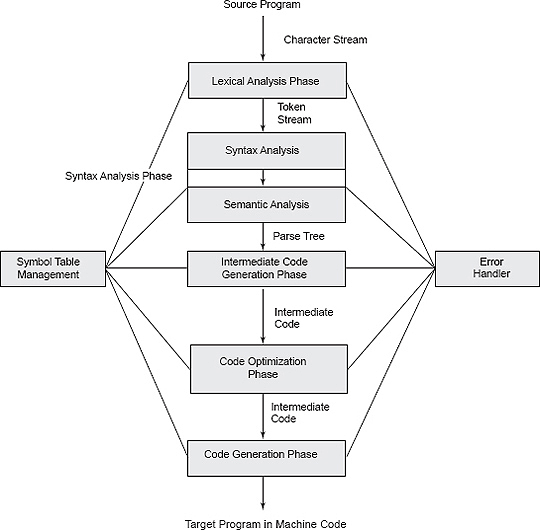
\includegraphics[width=1\textwidth]{resources/compilerStructure.jpg}
	\end{center}
	\caption{Zgradba prevajalnika \cite{compilerStructure}.}
	\label{pic1}
\end{figure}

Da lahko prevajalnik program prevede iz ene oblike v drugo, ga najprej analizira, razume njegovo strukturo ter pomen, nato pa ga pretvori v drugačno obliko.  \\
Analizo programa običajno delimo na naslednje korake \cite{modernCompiler}:
\begin{enumerate}
	\item \textbf{Leksikalna analiza} (angl. \textit{lexical analysis}).
	\item \textbf{Sintaksna analiza} (angl. \textit{syntax analysis}).
	\item \textbf{Semantična analiza} (angl. \textit{semantic analysis}).
\end{enumerate}

Po končani analizi sledi sinteza programa v izhodni/ciljni jezik. Sintezo do vmesne kode sestavljata:
\begin{enumerate}
	\item \textbf{Izračun klicnih zapisov} (angl. \textit{frame evaluation}).
	\item \textbf{Generiranje vmesne kode} (angl. \textit{intermidiate code generation}).
\end{enumerate}

\subsection{Leksikalna analiza}

Leksikalni analizator kot vhod prejme tok znakov, kot izhod pa vrne tok v naprej definiranih simbolov. Simbol je običajno zgrajen iz imena, vrednosti (t. i. \textit{lexeme}) ter lokacije v izvorni datoteki \cite{modernCompiler}.

\subsubsection{Leksikalni simboli:}

Simbol je zaporedje znakov, ki ga interpretiramo kot samostojno enoto v slovnici programskega jezika \cite{modernCompiler}. \\ 
Tabela \ref{tabel:vrsteZetonov} prikazuje nekaj vrst simbolov ter primere. \\

\begin{table}
	\begin{center}
		\begin{tabular}{l|c|c}
			\textbf{vrsta simbola} & \textbf{angl.} & \textbf{primeri} \\ \hline\hline
			ime & identifier & 
\begin{lstlisting} 
    x foo bar		
thisIsAnIdentifier
\end{lstlisting} \\
			rezervirana beseda & keyword & 
\begin{lstlisting} 
while for if		
public override
\end{lstlisting} \\
			operator & operator & 
\begin{lstlisting} 
, . && = ==
\end{lstlisting} \\
			niz znakov & string & 
\begin{lstlisting} 
"this is a string" 
\end{lstlisting} \\
			znak & character &
\begin{lstlisting} 
'a' 'x' '@'
\end{lstlisting} \\
			celo št. & integer &
\begin{lstlisting} 
10 125 082
\end{lstlisting} \\
			decimalno št. & real &
\begin{lstlisting} 
201.5 3.14 1.2e10
\end{lstlisting} \\
		\end{tabular}
	\end{center}
	\caption{Primeri simbolov v programskem jeziku Java.}
	\label{tabel:vrsteZetonov}
\end{table}

Delovanje leksikalne analize si lahko na kratko ogledamo na primeru programa \ref{lst:atherisCode}: rezultat leksikalne analize je prikazan kot izpis \ref{lst:lexedSource}.

\renewcommand{\lstlistingname}{Program}
\begin{lstlisting}[caption={Primer programa v programskem jeziku Atheris.},label={lst:atherisCode}, captionpos=b]
	let x: Int
	let y: Int
	x * y
\end{lstlisting}

\renewcommand{\lstlistingname}{Izpis}
\begin{lstlisting}[caption={Rezultat leksikalne analize za program ~\ref{lst:atherisCode}.},label={lst:lexedSource},captionpos=b]
	[1:1-1:4] 		LET:let
	[1:5-1:6] 		IDENTIFIER:x
	[1:6-1:7] 		COLON::
	[1:8-1:11] 		IDENTIFIER:Int
	[1:11-1:12] 	NEWLINE:\n
	[2:1-2:4] 		LET:let
	[2:5-2:6]			IDENTIFIER:y
	[2:6-2:7] 		COLON::
	[2:8-2:11] 		IDENTIFIER:Int
	[2:11-2:12] 	NEWLINE:\n
	[3:1-3:2] 		IDENTIFIER:x
	[3:3-3:4] 		MUL:*
	[3:5-3:6] 		IDENTIFIER:y
	EOF:$
\end{lstlisting}

\subsection{Sintaksna analiza}

Druga faza prevajanja je sintaksna analiza (angl. \textit{syntax analysis} ali \textit{parsing}). Naloga te faze je, da zagotovi, da je napisan program slovnično pravilen in v skladu s pravili sintakse. Sintaksni analizator prejme kot vhod tok simbolov, ki ga zgenerira prejšnja faza, rezultat pa je abstraktno sintaksno drevo. \\

\noindent\textbf{Abstraktno sintaksno drevo} (AST) je drevesna podatkovna struktura, ki predstavlja sintaksno strukturo programa. Vsako vozlišče drevesa ponazarja konstrukt v programski kodi.

\begin{figure}[h]
	\begin{center}
		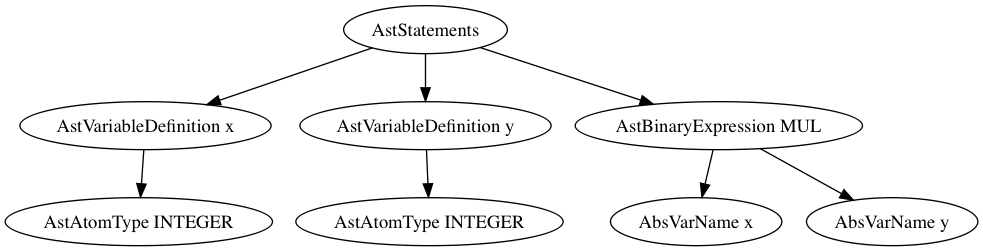
\includegraphics[width=1\textwidth]{resources/ast.png}
	\end{center}
	\caption{Abstraktno sintaksno drevo za program ~\ref{lst:atherisCode}.}
	\label{image:abstractSyntaxTree}
\end{figure}

Iz slike \ref{image:abstractSyntaxTree} lahko razberemo, da gre za dve definiciji spremenljivk in njuno množenje.\\\\
\indent Abstraktno sintaksno drevo je bistvenega pomena, saj nadaljnje faze operirajo izključno nad njim.

\subsection{Semantična analiza} \label{semanSection}

Semantična analiza poveže definicije spremenljivk z njihovimi uporabami ter preveri, ali so vsi izrazi pravilnih podatkovnih tipov \cite{modernCompiler}. \\
\indent Običajno izvedbo semantične analize razdelimo na dve podfazi:
\begin{enumerate}
	\item \textbf{Razreševanje imen:} zagotovi, da znotraj trenutnega območja vidnosti za vsako uporabo imena obstaja definicija z istim imenom, ter uporabo poveže z definicijo. \\
	Kot primer lahko navedemo program \ref{lst:atherisCodeNameError}, kjer se sklicujemo na nedefinirano spremenljivko, kar mora semantični analizator odkriti kot napako.
	\renewcommand{\lstlistingname}{Program}
	\begin{lstlisting}[caption={Primer programa, kjer spremenljivka \textit{y} ni definirana.}, label={lst:atherisCodeNameError},captionpos=b]
	let x: Int
	print(y)
	\end{lstlisting}
	
	\item \textbf{Preverjanje tipov:} vsakemu vozlišču v AST določi podatkovni tip ter na podlagi postavljenih semantičnih pravil zagotovi, da so vsi izrazi pravilnih tipov. \\
	Primer napake v fazi preverjanja tipov je prikazan s programom \ref{lst:atherisCodeTypeError}; operacija '+' ni definirana nad podatkovnima tipoma {\ttfamily Int} in {\ttfamily String}, zato semantični analizator javi napako.
	
	\renewcommand{\lstlistingname}{Program}
	\begin{lstlisting}[caption={Primer programa, kjer je napaka v podatkovnih tipih.},label={lst:atherisCodeTypeError},captionpos=b]
	let x: Int
	let s: String
	x + s
	\end{lstlisting}
	
\end{enumerate}

V zahtevnejših prevajalnikih se lahko tekom semantične analize opravi še dosti drugih analiz, npr. analizo inicializiranosti spremenljivk, zaznavanje mrtve kode, eliminacijo neuporabljenih izrazov ipd., vendar se z njimi v tem diplomskem delu ne ukvarjamo.

\begin{figure}[h]
	\begin{center}
		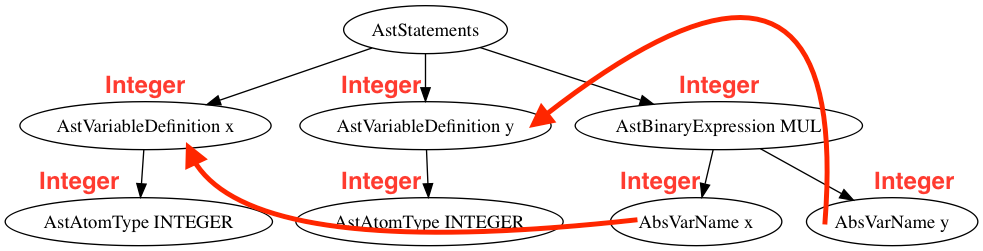
\includegraphics[width=1\textwidth]{resources/astSeman.png}
	\end{center}
	\caption{Rezultat semantične analize za program ~\ref{lst:atherisCode}.}
	\label{image:astSeman}
\end{figure}

Pri implementaciji semantične analize nam pomaga \textit{simbolna tabela}.

\subsubsection{Simbolna tabela}

Simbolna tabela je podatkovna struktura, ki preslika imena v njihove definicije in podatkovne tipe \cite{modernCompiler}. Ker običajno programi vsebujejo več tisoč definicij imen, mora podatkovna struktura omogočati učinkovito poizvedovanje. Iz slike ~\ref{image:astSeman} lahko razberemo, kaj se med izvajanjem semantične analize zgodi v ozadju: puščice predstavljajo povezave med definicijami in uporabami posameznih imen, evaluacija podatkovnih tipov pa je pri vseh vozliščih {\ttfamily Integer}, razen pri korenu, ki nima tipa oz. je tipa {\ttfamily Void}.\\
\indent Semantična analiza zagotovi, da za vsako uporabo imena obstaja njena definicija, in da so podatkovni tipi pravilni. Sliki \ref{image:astSemanCodeNameError} in \ref{image:astSemanTypeError} prikazujeta semantični napaki.

\begin{figure}[h]
	\begin{center}
		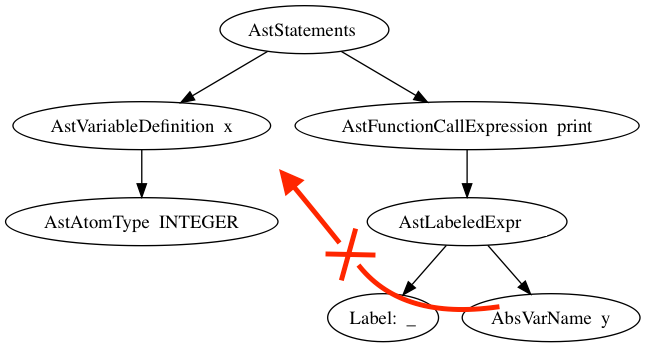
\includegraphics[width=0.9\textwidth]{resources/astSemanNameError.png}
	\end{center}
	\caption{Napaka v programu ~\ref{lst:atherisCodeNameError}; spremenljivka \textit{y} ni definirana.}
	\label{image:astSemanCodeNameError}
\end{figure}

\begin{figure}[h]
	\begin{center}
		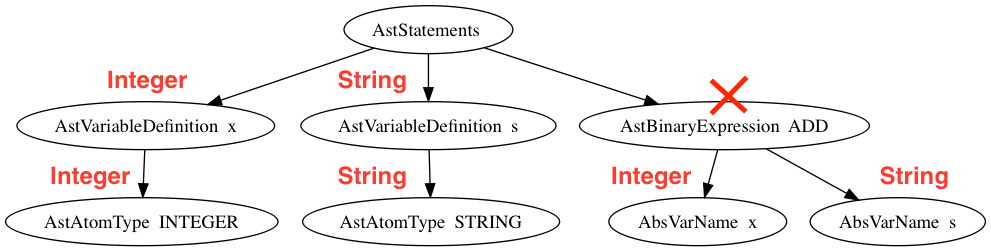
\includegraphics[width=1\textwidth]{resources/astSemanTypeError.png}
	\end{center}
	\caption{Napaka v programu ~\ref{lst:atherisCodeTypeError}; seštevanje med podatkovnima tipoma \textit{Integer} in \textit{String} ni dovoljeno.}
	\label{image:astSemanTypeError}
\end{figure}

\subsection{Klicni zapisi}

Klicni zapis je prostor v pomnilniku, ki vsebuje vse potrebne informacije za izvedbo posameznega klica funkcije. Običajno klicni zapis vsebuje prostor za lokalne spremenljivke, vhodne parametre in register, kamor se shrani izhodna vrednost funkcije. Zgradbo klicnega zapisa si lahko podrobneje ogledamo na sliki \ref{image:stackFramesImg}. \\
\indent V skoraj vsakem modernem programskem jeziku ima lahko funkcija \textit{lokalne} spremenljivke. Ker lahko hkrati obstaja več klicev iste funkcije, je pomembno, da ima vsak klic dostop do lastnih spremenljivk. Ta problem rešujemo s klicnimi zapisi \cite{modernCompiler}.  \\\\
\indent V funkciji 

\renewcommand{\lstlistingname}{Program}
\begin{lstlisting}
	func fib(_ n: Int) Int {
	    if n < 2 {
	        return 1
	    }
	    else {
	        return fib(n - 1) + fib(n - 2)
	    }
	}
	fib(10)
\end{lstlisting}
%
se za vsak njen klic ustvari nova instanca spremeljivke \textit{n}, ki živi na klicnem zapisu funkcije, vrednost pa ji priredimo kot vhodni argument. Ker je funkcija rekurzivna, živi v pomnilniku naenkrat veliko instanc spremenljivke \textit{n}, vsaka v lastnem klicnem zapisu \cite{modernCompiler}.

\begin{figure}[h]
	\begin{center}
		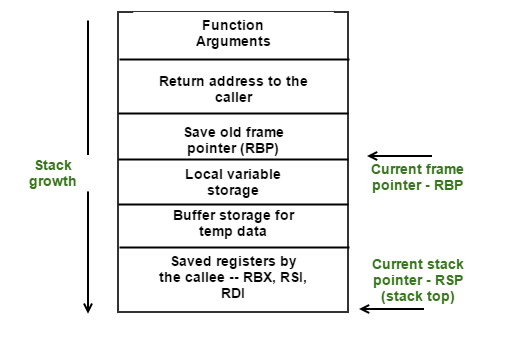
\includegraphics[width=0.9\textwidth]{resources/stackFrame.png}
	\end{center}
	\caption{Klicni zapis \cite{stackFrames}.}
	\label{image:stackFramesImg}
\end{figure}

\subsubsection{Sklad}

Klicni zapisi funkcij se shranjujejo na sklad. Sklad je v pomnilniku predstavljen kot velika tabela s posebnim registrom, imenovanim \textbf{skladovni kazalec} (angl. \textit{stack pointer}), ki kaže na konec sklada. Ob vsakem klicu funkcije se sklad poveča za velikost klicnega zapisa klicane funkcije. Podobno se ob vrnitvi funkcije zmanjša za enako vrednost \cite{modernCompiler}. 

\paragraph{Kazalec na klicni zapis:}

Predpostavimo da funkcija \textit{g} kliče funkcijo \textit{f}. Ob vstopu v f skladovni kazalec (SP) kaže na prvi vhodni argument funkciji f. Nov prostor na skladu je rezerviran tako, da se od SP odšteje velikost klicnega zapisa f. Tako SP sedaj kaže na konec sklada. Stara vrednost SP postane nova vrednost kazalca na klicni zapis (angl. \textit{frame pointer}). V programskih jezikih, kjer je velikost klicnega zapisa za posamezno funkcijo konstantna, je vrednost kazalca na klicni zapis (FP) vedno izračunljiva, zato si je ni potrebno posebej shranjevati na sklad \cite{modernCompiler}: 

\begin{lstlisting}
		FP = SP + velikost klicnega zapisa
\end{lstlisting}

\paragraph{Prenos parametrov:}

Standardni način klicanja funkcij je, da klicoča funkcija rezervira prostor na skladu za prenosih njenih izhodnih parametrov (oz. vhodnih parametrov za klicano funkcijo) \cite{modernCompiler}. \\ 
\indent Prostor za njih se običajno nahaja pred SP. Klicana funkcija tako naslov njenega i-tega parametra izračuna z enačbo
\begin{lstlisting}
		argumentAddress(i) = FP + (4 * i)
\end{lstlisting}

\paragraph{Statična povezava:}

V jezikih, ki podpirajo gnezdenje funkcij, lahko gnezdene funkcije dostopajo do spremenljivk, ki se nahajajo v zunanjih funkcijah. Da lahko gnezdena funkcija dostopa do spremenljivk, ki niso na njenem klicnem zapisu, ji ob klicu poleg ostalih parametrov posredujemo FP funkcije, ki jo neposredno definira. Temu kazalcu rečemo statična povezava (angl. \textit{static link}). 

\renewcommand{\lstlistingname}{Program}
\begin{lstlisting}[caption={Primer gnezdenih funkcij.}, captionpos=b, label={lst:nestedFunctions}]
    func f() {
        var x: Int = 10
        func e() {
            var z: Int = 100
        }
        func g() {
            var y: Int = 20
            func h() {
                print(x)
                print(y)
            }
        }
    }
\end{lstlisting}

Program ~\ref{lst:nestedFunctions} vsebuje gnezdeni funkciji \textit{g} in \textit{h}. Funkcija h lahko dostopa do spremenljivk definiranih v \textit{g} in \textit{f}, ne pa tudi do tistih v \textit{e}.

\subsection{Generiranje vmesne kode}   

\subsubsection{Vmesna koda}

Vmesna koda (angl. \textit{intermidiate representation}) je abstraktni približek strojne kode, a brez mnogih podrobnosti posameznih strojnih jezikov. Vmesna koda (IR) predstavlja ukaze, brez da bi poznali arhitekturo ciljne naprave. Poleg tega je vmesna koda neodvisna od izvornega jezika \cite{modernCompiler}. \\
\indent Dobra predstavitev vmesne kode ima naslednje lastnosti \cite{modernCompiler}:

\begin{enumerate}
	\item Njeno generiranje mora biti priročno.
	\item Pretvorba vmesne kode v dejansko strojno kodo mora biti priročna za vse ciljne arhitekture.
	\item Vsak gradnik mora imeti jasen pomen, da so lahko optimizacijske transformacije enostavno implementirane.
\end{enumerate}

Poznamo dve vrsti vmesne kode: drevesno in linearno. Za linearno vmesno kodo se pogosto uporablja t. i. \textit{three-address code} (TAC ali 3AC), kar pomeni, da imajo lahko ukazi take kode največ tri operande. \\
\indent Pri predmetu smo uporabili drevesno vmesno kodo, zato je tudi vmesna koda, zgenerirana s strani prevajalnika za Atheris, drevesna.\\
\indent Posamezni deli abstraktnega sintaksnega drevesa so lahko kompleksne stvari, na primer zanke, klici funkcij itd., ki jih ne moremo neposredno preslikati v strojne ukaze. Zato morajo gradniki vmesne kode predstavljati le enostavne operacije, kot so npr. LOAD (preberi vrednost iz pomnilnika), STORE (shrani vrednost v pomnilnik), ADD (seštej dve vrednosti) itd. Tako lahko vsak posamezni del AST prevedemo v pravo zaporedje ukazov abstraktne vmesne kode \cite{modernCompiler}. \\ 

\chapter{Programski jezik PINS}

Programski jezik PINS je učni programski jezik, zato je tudi dokaj preprost. Prevajalnik zanj smo implementirali v sklopu domačih nalog pri predmetu Prevajalniki in navidezni stroji.

\section{Leksikalna pravila}

Programski jezik PINS podpira tri atomarne podatkovne tipe: {\ttfamily integer},  {\ttfamily logical}, {\ttfamily string}, za katere so rezervirane istoimenske besede. Celoštevilske konstante so poljubno predznačeno zaporedje števk, logične konstante so ali {\ttfamily true} ali {\ttfamily false}, znakovne konstante pa so definirane kot poljubno (lahko prazno) zaporedje znakov z ASCII kodami med vključno 32 in 126, ki je obdano z enojnima navednicama (ASCII koda 39); izjema je en sam enojni narekovaj, ki je podvojen. \\
\indent Imena so definirana kot poljubno zaporedje črk, številk in podčrtajev, ki se ne začne s številko in ni rezervirana beseda ali kakšna od prej naštetih konstant. \\
\indent Belo besedilo (angl. \textit{whitespace}) so presledki (ASCII 32), tabulatorji (ASCII 9) in znaka za konec vrstice (ASCII 10 in 13). \\
\indent Komentarji se začnejo z {\ttfamily \#} (ASCII 35) in se raztezajo do konca vrstice.

\section{Sintaksna pravila} \label{pinsSyntax}

Celotna izvorna koda je sestavljena iz seznama definicij. Vsaka definicija je lahko:

\begin{enumerate}
	\item Definicija tipa (oz. sklic na tip - \textit{typealias}).
	\item Definicija spremenljivke.
	\item Definicija funkcije.
\end{enumerate}

Kot smo že omenili, PINS podpira tri osnovne podatkovne tipe, vendar sintaksa omogoča tudi definicijo tabel (angl. \textit{array}) s fiksno velikostjo. \\
\indent Definicija funkcije je sestavljena iz imena, seznama parametrov, tipa, ki ga funkcija vrača, ter \textit{izraza} oz. jedra funkcije. Zanimivo pri PINS-u je to, da izven jedra funkcij ne moremo početi ničesar drugega, kot ustvarjati definicije (podobno kot pri Javi). \\
\indent S stališča sintaksne analize je izraz (angl. \textit{expression}) lahko:
\begin{enumerate}
	\item Logični izraz
	\item Primerjalni izraz
	\item Seštevalni izraz
	\item Multiplikativni izraz
	\item Prefiksni izraz
	\item Postfiksni izraz
	\item Atomarni izraz
\end{enumerate}

Za uspešno izvedbo sintaksne analize je atomarni izraz lahko:
\begin{enumerate}
	\item Logična konstanta
	\item Celoštevilska konstanta
	\item Znakovna konstanta
	\item Ime
	\item Klic funkcije
	\item If stavek
	\item If else stavek
	\item While stavek
	\item Zaporedje izrazov
\end{enumerate}

Moramo se zavedati, da sestavljeni stavki, ki smo jih našteli kot atomarne izraze, seveda niso nedeljivi s stališča jezika. Med atomarne izraze so vključeni zaradi upoštevanja prioritet aritmetičnih in logičnih operatorjev. Vsakemu izrazu lahko sledijo tudi definicije, ki so gnezdene znotraj zavitih oklepajev.

\section{Semantična pravila}

\subsubsection{Območja vidnosti}

Imena so vidna v celotnem območju vidnosti, ne glede na mesto definicije. Izraz {\ttfamily expression \{ WHERE definitions \}} ustvari novo vgnezdeno območje vidnosti. To pomeni, da definicije znotraj zavitih oklepajev niso vidne navzven. Tudi definicija funkcije ustvari novo vgnezdeno območje vidnosti, ki se začne za imenom in se razteza do konca funkcije.

\subsubsection{Tipiziranost}

\begin{enumerate}
	\item \textit{integer}, \textit{logical}, \textit{string} opisujejo podatkovne tipe INTEGER, LOGICAL in STRING, zaporedoma
	\item izraz 
\begin{lstlisting}[]
	arr [ n ] type
\end{lstlisting}
	opisuje podatkovni tip ARR(n, type), kjer je \textit{n} celoštevilska konstanta 
\end{enumerate}

\subsubsection{Deklaracije}

\begin{enumerate}
	\item Deklaracija tipa
\[
typ\quad  identifier\quad  :\quad  type
\]
	ustvari sklic na podatkovni tip \textit{type} z imenom \textit{identifier}
	\item Deklaracija funkcije
%\begin{lstlisting}[]
\[ fun\quad identifier  ( identifier_1 : type_1, ..., identifier_n : type_n ) : type = expression \]
%\end{lstlisting}
	določa funkcijo, ki je tipa \[type_1 \quad *, \quad  ..., \quad *\quad  type_n \,\to\, type \]
	\item Deklaracija spremenljivke
\[
var \quad identifier\quad :\quad type
\]

določa spremeljivko tipa $type$
	\item Deklaracija parametra
\[
identifier \quad :\quad type
\]
določa parameter tipa $type$
\end{enumerate}

\section{Primeri}

Programa \ref{lst:bubblePins} in \ref{lst:fibonacciPins} prikazujeta primera podprogramov napisanih v programskem jeziku PINS (celotni programi se nahajajo v prilogi \ref{primeriPins}).

\begin{lstlisting}[caption={Sortiranje z navadnimi zamenjavami.}, captionpos=b, label={lst:bubblePins}]
	fun bubble(tab: arr[13] integer) : integer = (
	    {for i = 0, 13, 1 :
	        {for j = 0, 13, 1:
	            {if tab[j] > tab[i] then 
	            (
	                {tmp = tab[j]},
	                {tab[j] = tab[i]},
	                {tab[i] = tmp}, 0
	            ) 
	            { where var tmp : integer} }
	    	}
		},
		1
	) { where var i : integer; var j : integer };
\end{lstlisting}

\begin{lstlisting}[caption={Izračun n-tega fibonaccijevega števila.}, captionpos=b, label={lst:fibonacciPins}]
	fun fib(x: integer) : integer = (
	    { if x < 2 then
	        ({rez = 1})
	    else 
	        ({rez = fib(x - 1) + fib(x - 2)})
	    },
	    rez
	) {where var rez : integer};
\end{lstlisting}

\chapter{Programski jezik Atheris}
\label{ch1}

Programski jezik Atheris je programski jezik, ki je nastal kot nadgranja programskega jezika PINS. \\
\indent Kljub temu, da prevajalnik za Atheris izhaja iz prevajalnika za PINS, se jezika med seboj zelo razlikujeta. Atheris vsebuje veliko nadgradenj napram PINSu, poleg tega pa se razlikujeta tudi v sintaksi, ki je v programskem jeziku Atheris zelo podobna sintaksi programskega jezika Swift. 
\begin{figure}[h]
	\begin{center}
		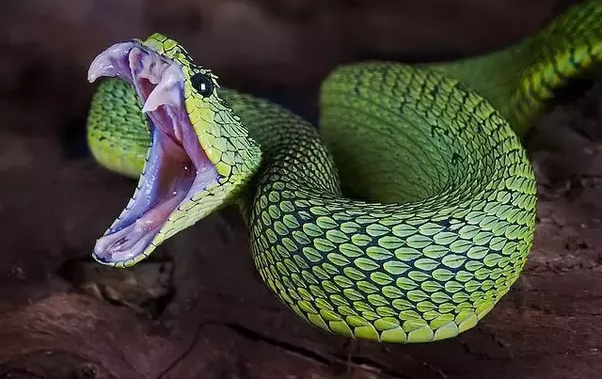
\includegraphics[width=1\textwidth]{resources/atheris.png}
	\end{center}
	\caption{Atheris Chlorechis (West African bush viper) \cite{Atheris}.}
	\label{image:ast}
\end{figure}

\noindent Razlike med jezikoma so vidne v prilogi, ki vsebuje rešitve za tri znane probleme napisane v obeh jezikih. \\
\indent Med drugim nova sintaksa omogoča definiranje kompleksnejših podatkovnih tipov z uporabo razredov, vmesnikov, terk in enumeracij. \\
\indent Posamezni stavki so med seboj ločeni z novimi vrsticami (Python, Swift), vendar pa prevajalnik omogoča njihovo ločevanje tudi s podpičjem {\ttfamily ;} (C++, Java). \\
\indent Komentarji se lahko začnejo bodisi z {\ttfamily \#} in se raztezajo do konca vrstice (Python, PINS), bodisi z {\ttfamily /*} in končajo z {\ttfamily */} (Java, C++). \\
\indent Podprt je tudi {\ttfamily switch} kontrolni stavek. \\
\indent Definicije funkcij ter klici funkcij so spremenjeni; parametri funkcije so sedaj sestavljeni iz labele ter imena parametra (tako kot v Swiftu). Pri klicu funkcije se uprabi labela parametra, znotraj jedra funkcije pa se uporablja ime.

\subsection{Podatkovni tipi}

Podprti atomarni podatkovni tipi so: {\ttfamily integer, double, string, char} in {\ttfamily bool}. Podprti so tudi kompleksni podatkovni tipi:

\begin{enumerate}
	\item Enumeracije
	\item Terke
	\item Razredi
	\item Vmesniki
\end{enumerate} 

\indent Podatkovni tipi spremenljivk, ki jim priredimo objekt, terko ali tabelo, se implicitno smatrajo kot kazalci, kar ni razvidno iz same sintakse jezika. Ena izmed prednosti kazalcev je v tem, da pri prenosu objekta kot argument funkciji le-tega ni potrebno v celoti kopirati na sklad, ampak posredujemo le njegov naslov v pomnilniku. Velikost klicnega zapisa je zaradi tega lahko manjša, hkrati pa je izvedba funkcije hitrejša.

\section{Sintaksa}

Celoten program v jeziku PINS je sestavljen iz seznama definicij, kje je definicija lahko definicija spremenljivke, definicija tipa ali definicija funkcije. Sintaksa programskega jezika Atheris se razlikuje v tem, da je program sestavljen iz zaporedja stavkov, stavki pa se delijo na \textit{izraze} in \textit{definicije}. \\
\indent Definicije so predstavljene z naslednjimi konteksno neodvisnimi gramatikami (KNG):
 
\begin{enumerate}
	\item Spremenljivke
\begin{lstlisting}[]
var_def -> var identifier 
var_def -> var identifier = expr
var_def -> var identifier: type 
var_def -> var identifier: type = expr 
\end{lstlisting}
	\item Funkcije
\begin{lstlisting}[]
func_def -> prototype { statements }

prototype -> func identifier ( parameters )
prototype -> func identifier ( parameters ) type

parameters -> $
parameters -> paramater
parameters -> paramaters, paramater

parameter -> identifier : type
parameter -> identifier identifier : type
\end{lstlisting}	
	\item Enumeracije
	
\begin{lstlisting}
enum_def -> enum { enum_defs }

enum_defs -> $
enum_defs -> enum_member_def
enum_defs -> enum_defs, enum_member_def

enum_member_def -> case identifier
enum_member_def -> case identifier = expression
\end{lstlisting}
	\item Razredi
\begin{lstlisting}
class_def -> class { definitions }
\end{lstlisting}

\end{enumerate} 

Sintaksa izrazov je skoraj identična PINSu (\ref{pinsSyntax}), razen izrazov za nadzor toka (angl. \textit{control flow}):

\begin{enumerate}
	\item If stavek
\begin{lstlisting}[]
if_expr -> if expr { statements } else_ifs
			
else_ifs -> $
else_ifs -> else if { statements } else_ifs
else_ifs -> else { statements }
\end{lstlisting}
	\item Switch stavek
\begin{lstlisting}[]
switch_expr -> switch expr { cases }

cases -> $
cases -> case tuple_exprs: statements cases
cases -> default: statements

tuple_exprs -> expr
tuple_exprs -> expr, tuple_exprs
\end{lstlisting}
	\item While stavek
\begin{lstlisting}[]
while_expr -> while expr { statements }
\end{lstlisting}
	\item For stavek
\begin{lstlisting}[]
for_expr -> for identifier in expr { statements }
\end{lstlisting}
	\item Terka
\begin{lstlisting}
tuple_expr -> ( tuple_exprs )

tuple_exprs -> expr
tuple_exprs -> tuple_exprs, expr
\end{lstlisting}
\end{enumerate} 

Kot smo že omenili, sintaksa programskega jezika Atheris omogoča, da so posamezni stavki ločeni bodisi s {\ttfamily ;} bodisi z novo vrstico. Za ta namen je dodana nova vrsta simbolov, ki predstavlja novo vrstico v izvorni kodi (pred tem se je znak za novo vrstico štel kot belo besedilo). V primeru, da je v izvorni kodi več zaporednih novih vrstic, jih leksikalni analizator požre in vedno vrne samo en zaporedni \textit{newline} simbol. To naredi sintaksno analizo enostavnejšo. 

\section{Funkcije}

Ob deklaraciji funkcije lahko opcijsko definiramo poljubno število poimenovanih ter tipiziranih vrednosti, ki jim skupaj rečemo parametri funkcije. Poleg tega lahko opcijsko navedemo še podatkovni tip vrednosti, ki jo bo funkcija vračala (privzeto funkcije ne vračajo ničesar – {\ttfamily Void}).\\
\indent Programski jezik Atheris zahteva, da ob klicu funkcij poleg imena funkcije navedemo tudi imena parametrov. \\
\indent Imena parametrov so sestavljena iz dveh delov: labele argumenta ter imena parametra. Labele argumentov se uporabljajo ob klicu funkcije, medtem ko se imena parametrov uporabljajo znotraj jedra funkcije. Labele so privzeto identične imenom. \\\indent Primer funkcije ter njenega klica si lahko ogledamo na programu \ref{lst:functions1}.

\begin{lstlisting}[caption={Primer definicije in klica funkcije.}, captionpos=b, label={lst:functions1}]
	func someFunction(firstParameterName: Int, 
									  secondParameterName: Int) 
	{
	  /* znotraj telesa funkcije, sta firstParameterName in secondParameterName referenci na  vrednosti argumentov za prvi in drugi parameter. */
	}
	someFunction(firstParameterName: 1, 
							 secondParameterName: 2)
\end{lstlisting}

\subsection{Določanje label argumentov}

Če želimo, da sta labela in ime različna, navedemo labelo argumenta pred imenom, kot je razvidno iz programa \ref{lst:functions2}.

\begin{lstlisting}[caption={Labela argumenta in ime parametra se razlikujeta.}, captionpos=b, label={lst:functions2}]
	func someFunction(argumentLabel parameterName: Int) 
	{
		/* znotraj telesa funkcije, se parameterName sklicuje na vrednost argumenta funkciji */
		print(parameterName)
	}
	someFunction(argumentLabel: 1)
\end{lstlisting}

Podprta je tudi možnost, da se izognemo navajanju imen argumentov pri klicanju funkcij. To storimo tako, da označimo labelo argumenta z '\_', kar prikazuje program \ref{lst:functions3}.

\begin{lstlisting}[caption={Klic funkcije brez navedbe imen argumentov.}, captionpos=b, label={lst:functions3}]
	func someFunction(_ firstParameterName: Int, 
									  _ secondParameterName: Int) {}
	someFunction(1, 2)
\end{lstlisting}

Opisane funkcionalnosti so implementirane tako, da se v simbolno tabelo ne shrani samo ime funkcije, kot je stvar realizirana v prevajalniku za PINS, ampak se celotna definicija fukcije, oz. njen prototip, pretvori v posebno znakovno predstavitev, ki je sestavljena iz imena ter label argumentov.

\renewcommand{\lstlistingname}{Izpis}
\begin{lstlisting}[caption={Znakovne predstavitve funkcij.}, captionpos=b, label={lst:functionStringRepr}]
someFunction(firstParameterName:secondParameterName:)
someFunction(argumentLabel:)
someFunction(_:_:)
\end{lstlisting}

Tako imenovano \textit{overloadanje} funkcij sedaj ni problem, saj čeprav imajo funkcije ista imena, se na vsako izmed njih sklicujemo preko različne predstavitve, zato jih lahko v simbolni tabeli ustrezno poiščemo. Seveda je potrebno v podobni obliki predstaviti tudi klice funkcij. \\
\indent Znakovne predstavitve funkcij iz prejšnjih primerov si lahko ogledamo na izpisu \ref{lst:functionStringRepr}.

\section{Enumeracije}

Enumeracija je podatkovna struktura, ki definira skupen tip skupini povezanih vrednosti in olajša delo nad njimi. Enumeracija vsebuje poljubno število vrednosti/konstant, ki jim lahko priredimo tako imenovane \textit{surove vrednosti}. Podatkovni tip surovih vrednosti definiriamo v naprej in je pri vseh konstantah enak. \\
\indent V primeru, da enumeracija vsebuje surove vrednosti, jih je potrebno eksplicitno navesti za vse konstante enumeracije. Izjema so surove vrednosti za podatkovna tipa {\ttfamily Int} in {\ttfamily String}. \\
\indent Privzeto so surove vrednosti za {\ttfamily Int} zaporedna števila začenši z 0. V primeru, da je vrednost eksplicitno navedena, je vrednost naslednje surove vrednosti naslednje zaporedno število od prejšnje vrednosti. \\
\indent Definirajmo enumeracijo, ki modelira dneve v tednu s surovimi vrednostmi tipa {\ttfamily Int}:

\renewcommand{\lstlistingname}{Program}
\begin{lstlisting}[caption={}, captionpos=b]
	enum Days: Int {
	  case Monday # vrednost = 0
	  case Tuesday = 10 # vrednost = 10
	  case Wednesday # vrednost = 11
	  case Thursday = 100 # vrednost = 100
	  case Friday # vrednost = 101
	}
\end{lstlisting}

\indent Če je podatkovni tip surovih vrednosti {\ttfamily String}, je njihova privzeta vrednost kar ime konstante, kot je razvidno iz programa \ref{lst:fruitEnumeration}.

\begin{lstlisting}[caption={Enumeracija s surovimi vrednostmi tipa String.}, captionpos=b, label={lst:fruitEnumeration}]
	enum Fruit: String {
	  case Apple # privzeta vrednost = "Apple"
	  case Orange = "Annoying Orange"
	  case Strawberry # privzeta vrednost = "Strawberry"
	}
\end{lstlisting}

\indent Če enumeracija ne vsebuje surovih vrednosti, je semantična analiza dokaj preprosta. V primeru, da so surove vrednosti prisotne, postane kompleksnejša, saj je potrebno zagotoviti, da so ustreznega podatkovnega tipa. Poleg tega je potrebno določiti implicitne surove vrednosti konstant, če niso eksplicitno navedene. \\
\indent Do posameznih elementov enumeracije dostopamo z \textit{DOT} operatorjem ({\ttfamily .}), kjer je na levi strani ime enumeracije, na desni pa ime elementa. Operator {\ttfamily .} zagotovi, da se v sestavljenem podaktovnem tipu na levi strani nahaja član z imenom na desni strani (več o operatorju v nadaljevanju). Podobno dostopamo tudi do surovih vrednosti z uporabo imena {\ttfamily rawValue}. \\
\indent Dostop do konstant enumeracije je prikazan v programu \ref{lst:fruitEnumerationUsage}.

\begin{lstlisting}[caption={Izpis surovih vrednosti enumeracije ~\ref{lst:fruitEnumeration}.}, captionpos=b, label={lst:fruitEnumerationUsage}]
	print(Fruit.Apple.rawValue) # 'Apple'
	print(Fruit.Orange.rawValue)  # 'Annoying Orange'
	print(Fruit.Strawberry.rawValue)  # 'Strawberry'
\end{lstlisting}

Kot je razvidno iz programa \ref{lst:enumUsage1}, lahko konstante enumeracij prirejamo spremenljivkam ter nad njimi izvajamo logični operaciji primerjanja vrednosti.

\begin{lstlisting}[caption={Prireditev konstante enumeracije spremenljivki.}, captionpos=b, label={lst:enumUsage1}]
	let x: Languages = Languages.Cpp
	if x == Languages.Java {
	    print("Java")
	}
	else {
	    print("Some other language")
	}
\end{lstlisting}

\section{Terke}

Terka je podatkovna struktura sestavljena iz poljubnega števila elementov, ki so lahko različnih podatkovnih tipov. Terke poznajo jeziki, kot sta Python in Swift, medtem ko jih Java in C++ ne poznata. Primera terk v programskem jeziku Atheris si lahko ogledamo na primerih \ref{lst:tuple1} in \ref{lst:tuple2}. \\
\indent Terka je definirana kot zaporedje izrazov znotraj oklepajev. Do posameznih elementov terke dostopamo na enak način kot dostopamo do članov enumeracije, ime elementa pa je njegov indeks v terki. 

\begin{lstlisting}[caption={Terka, sestavljena iz dveh vrednosti ({\ttfamily Int}, {\ttfamily Double}).}, captionpos=b, label={lst:tuple1}]
	let x = (10, 5.5)
	print(x.0)
	print(x.1)
\end{lstlisting}

Vsakemu izrazu znotraj terke lahko opcijsko določimo tudi ime. V primeru, da ime ni eksplicitno določeno, se za ime uporabi indeks (začenši z 0).

\begin{lstlisting}[caption={Terka s poimenovanim elementom.}, captionpos=b, label={lst:tuple2}]
	let x = (lorem: "Lorem", "Ipsum")
	print(x.lorem)
	print(x.1)
	# print(x.0) - napaka
\end{lstlisting}

\indent V pomnilniku so terke predstavljene skoraj identično kot tabele z razliko, da se podatkovni tipi elementov med sabo lahko razlikujejo. Ravno zaradi tega ne moremo odmika izračunati na enak način kot pri tabelah, kjer indeks pomnožimo z velikostjo podatkovnega tipa. \\
\indent Odmik posameznega elementa v terki izračunamo kot vsoto velikosti podatkovnih tipov vseh elementov pred želenim elementom:

\vspace{-5mm}
\[ offset ( element_i )  = sum ( size ( element_0 ), size( element_1 ), ..., size ( element_{i-1})) \]

Terke se pogosto uporabne v situacijah, kjer želimo, da funkcija vrne več vrednosti hkrati (funkcija seveda še vedno vrača le eno vrednost, tj. naslov, kjer se nahaja terka). \\
\indent Definirajmo funkcijo, ki evaluira polje igre tri v vrsto, in vrne dve vrednosti - naslednjo pozicijo kamor naj igralec igra ter stanje igre.

\begin{lstlisting}[caption={}, captionpos=b]
	func evaluateBoard(_ ticTacToe: [Char]) (Int, Int) {
	    return (1, 10)
	}
	let eval = evaluateBoard(['X', ' ', 'X'])
	print(eval.0) # '1'
	print(eval.1) # '10'
\end{lstlisting}

\section{Razredi}

Razred je sestavljena podatkovna struktura, ki, podobno kot terka, v sebi hrani spremenljivke različnih podatkovnih tipov. Vsak razred lahko vsebuje poljubno število atributov (spremenljivk) ter poljubno število metod – to so člani rezreda. \\
\indent Atributi in metode so lahko statični, kar pomeni, da niso del posamezne instance razreda, ampak živijo v statični instanci, ki je kreirana avtomatsko s strani prevajalnika. Poleg tega so lahko člani razreda \textit{privatni} ali \textit{javni}. Do privatnih članov ne moremo dostopati izven razreda. \\
\indent Poleg atributov in metod lahko razred vsebuje tudi definicije gnezdenih razredov, enumeracij ter vmesnikov.\\
\indent V pomnilniku je instanca razreda (objekt) predstavljena podobno kot terka, tj. kot tabela z vrednostmi različnih podatkovnih tipov. Zato tudi odmik elementov računamo na enak način. \\
\indent Primer definicije in uporabe razredov si lahko ogledamo v programu \ref{lst:nestedClassAth}.

\subsection{Dostop do članov in nadzor dostopa}

Do članov razreda dostopamo preko DOT operatorja. DOT operator je binarni operator in je sestavljen iz dveh izrazov, ki ju povezuje pika. \\
\indent Kot smo omenili se povezovanje definicij z njihovimi uporabami običajno opravi tekom faze razreševanja imen, kar pri sestavljenih podatkovnih strukturah (vključno z enumeracijami in terkami) ni mogoče. S tem se zato ne ukvarjamo tekom razreševanja imen, ampak problem prepustimo fazi razreševanja tipov. \\
\indent Razreševanje tipov za ta namen delimo na dve podfazi (dva sprehoda po AST). Cilj prvega sprehoda je evaluacija podatkovnih tipov definicij. Ko izračunamo podatkovne tipe vseh definicij v razredu, zgradimo sestavljen podatkovni tip, ki vsebuje podatke o vseh definicijah razreda in njihovih podatkovnih tipih. \\ 
\indent Cilj drugega sprehoda je razreševanje podatkovnih tipov izrazov. Ko prevajalnik naleti na operator {\ttfamily .} lahko sedaj poveže ime na desni z definicijo, ki se nahaja v sestavljenem podatkovnem tipu na levi strani.\\\\

\noindent \textbf{Nadzor dostopa}

\noindent Programski jezik Atheris trenutno pozna dva modifikatorja vidnosti: {\ttfamily public} in {\ttfamily private}. Modifikator public omogoča dostop do in spreminjanje vrednosti člana razreda kodi, ki se ne nahaja v razredu, za razliko od modifikatorja {\ttfamily private}, ki to prepoveduje. Privzeto so vsi člani razreda {\ttfamily public}. 
\subsection{Instančne funkcije}

Razred ima lahko v sebi definirane funkcije, ki se jim v OOP žargonu pogosto reče \textit{metode}. Metode se od funkcij razlikujejo v tem, da vsebujejo impliciten parameter, ki je referenca na objekt, ki metodo kliče.  \\
\indent Prevajalnik implicitni {\ttfamily self} parameter avtomatsko vstavi v vse metode razreda. Delno to stori tekom razreševanja imen, ko definiciji funkcije vstavi nov parameter, delno pa tekom razreševanja tipov, ko parametru nastavi tip razreda, v katerem je metoda definirana.

\subsection{Konstruktorji}

Konstruktorji so posebna vrsta metod in so odgovorni za kreacijo objektov ter inicializacijo atributov. Podobno kot ostalim metodam razreda, tudi konstruktorjem prevajalnik implicitno vstavi {\ttfamily self} parameter. \\
\indent Naloga konstruktorja je, da na kopici, tj. delu pomnilnika, kamor shranjujemo dinamično alicirane objekte (za razliko od sklada, kamor shranjujemo statične), alocira prostor, kjer bo shranjen objekt. Za dinamično alociranje pomnilnika se uporabi gradnik vmesne kode \textbf{ImcMALLOC}. Ta gradnik na kopici rezervira želeno velikost pomnilnika ter vrne naslov. \\ 
\indent Pri generiranju vmesne kode prevajalnik vstavi na začetek kode konstruktorja MALLOC gradnik, ki bo rezerviral prostor za objekt. Nato bo prevajalnik vrnjen naslov shranil na sklad v parameter {\ttfamily self}, zato da lahko znotraj konstruktorja nastavimo vrednosti ostalih atributov razreda. Na koncu bo ta naslov konstruktor tudi vrnil. Vrnjen naslov je referenca na objekt in ga uporabljamo za nadaljnje operacije nad njim. \\
\indent Razred ima lahko poljubno število konstruktorjev, ki jih definiramo z uporabo ključne besede {\ttfamily init}. Primere definicij konstruktorjev si lahko ogledamo na programih \ref{lst:constr1}, \ref{lst:constr2} in \ref{lst:constr3}. \\

\begin{lstlisting}[caption={Konsturktorji.}, captionpos=b, label={lst:constr1}]
	class Atheris {
	    var x: Int
	    init() {
	        self.x = 0
	    }
	    init(x: Int) {
	        self.x = x
	    }
	}
\end{lstlisting}

\indent Prevajalnik samodejno zgenerira impliciten \textit{privzeti} konstruktor, ki vsebuje kodo za inicializacijo atributov, ki jim nastavimo vrednost ob sami definiciji. 

\begin{lstlisting}[caption={Implicitni privzeti konstruktor.}, captionpos=b, label={lst:constr2}]
	class Atheris {
	    var x: Int = 10
	    var y: Int = 20
	}
	print(Atheris().x) # 10
	print(Atheris().y) # 20
\end{lstlisting}

V primeru, da je v razredu privzeti konstruktor tudi eksplicitno definiran, bo poleg svoje kode vseboval tudi kodo implicitnega.

\begin{lstlisting}[caption={Eksplicitni privzeti konstruktor.}, captionpos=b, label={lst:constr3}]
	class Atheris {
	    var x: Int = 10
	    var y: Int = 20
	    init() { # privzeti konstruktor
	        self.y = 100
	    }
	}
	print(Atheris().x) # 10
	print(Atheris().y) # 100
\end{lstlisting}

\subsection{Statični člani razreda}

Statični člani razreda so tisti člani, ki ne živijo znotraj posameznih instanc, ampak živijo v globalni statični instanci razreda. Definiramo jih z uporabo modifikatorja {\ttfamily static}. Statična instanca razreda je avtomatsko naložena v pomnilnik ob zagonu programa. Do statičnih članov dostopamo preko imena razreda. Ker statične funkcije niso del instance razreda, ne vsebujejo {\ttfamily self} parametra.

\begin{lstlisting}[caption={Klicanje statične funkcije.}, captionpos=b, label={lst:staticFunc}]
    class Static {
        static func foo() {
            print("I am a static function")
        }
    } 
	Static.foo()
\end{lstlisting}

\indent V času razreševanja tipov so statične definicije razreda shranjene v ločeno podatkovno strukturo od instančnih. Vozlišču AST, ki definira razred (\textit{AstClassDefinition}), v simbolno tabelo ne pripišemo \textit{razredni} podatkovni tip, ampak \textit{statični} tip, ki hrani podatke o statičnih definicijah razreda. Primer definicije in klicanja statične funkcije lahko vidimo v programu \ref{lst:staticFunc} \\
\indent Razredi lahko vsebujejo tudi enumeracije in gnezdene razrede. Definicije enumeracij in razredov se smatrajo kot statične, zato do njih dostopamo enako kot do statičnih članov. \\
\indent Definirajmo razred, ki vsebuje gnezdeno enumeracijo:

\begin{lstlisting}[caption={}, captionpos=b]
	class Static {
	    enum Languages: Int {
	        case Cpp, Java
	    }
	}
	let x = Static.Languages.Java
	print(x.rawValue) # '1'
\end{lstlisting}

Da lahko dostopamo do konstruktorjev znotraj gnezdenih razredov, jih prevajalnik avtomatično potisne v seznam statičnih metod razreda.

\begin{lstlisting}[caption={Definicija gnezdenega razreda in njegova uporaba.}, captionpos=b, label={lst:nestedClassAth}]
	class Main {
		class Person {
			var name: String
			var age: Int
		
			init(name: String, age: Int) {
				self.name = name
				self.age = age
			}
		}
		
		static func main(args: [String]) {
			let person = Person(name: args[1], age: 32)
			print(person.name)
			print(person.age)
		}
	}
	
	let args = ["Main.ar", "Janez Novak"]
	Main.main(args: args)
\end{lstlisting}

\section{Dedovanje in polimorfizem}

Dedovanje in polimorfizem sta, poleg enkapsulacije in abstrakcije, najpomembnejša koncepta OOP programiranja. Dedovanje je mehanizem, s katerim objekt pridobi (podeduje) nakatere ali vse lastnosti drugega objekta, medtem ko je polimorfizem sposobnost predstaviti isto funkcionalnost z različnimi implementacijami. Programski jezik Atheris omogoča enkratno dedovanje, tako kot Java in Swift. \\
\indent V pomnilniku se atributi dedovanega razreda nahajajo pred atributi dedujočega se razreda. Enačba za izračun velikosti razreda (koliko prostora porabi objekt v pomnilniku) postane kompleksnejša, saj je potrebno rekurzivno prišteti velikosti nadrazradov. Prav tako postane kompleksnejši izračun odmikov atributov od začetnega naslova.

\subsection{Polimorfizem}

Programski jezik Atheris omogoča, da razredi predstavijo lastne implementacije metod, ki se nahajajo v starševskem razredu. Vsako tako metodo moramo označiti z modifikatorjem {\ttfamily override}. Če želimo dedujočim se razredom preprečiti \textit{overridanje} metod, jim moramo dodati modifikator {\ttfamily final}.

\begin{lstlisting}[caption={Polimorfizem.}, captionpos=b, label={lst:virtualTableExamples}]
	class BaseClass {
	    func f1() {}
	    final func f2() {}
	}
	class DerivedClass: BaseClass {
	    override func f1() {}
	    # override func f2() {} - Ni dovoljeno
	}
\end{lstlisting}
%
Program \ref{lst:virtualTableExamples} demonstrira delovanje polimorfizma v programskem jeziku Atheris.

\subsection{Dinamično klicanje funkcij} \label{dynamicDispatch}

Dinamično klicanje funkcij (angl. \textit{dynamic dispatch}) je proces izbire, katera implementacija polimorfne operacije naj se izvede v času izvajanja programa. Običajno lahko že v času prevajanja izberemo, katera implementacija funkcije naj se kliče, saj obstaja samo ena. Pri razredih nastane problem, saj imajo lahko dedujoči se razredi svoje implementacije funkcij (oz. metod), kot je razvidno v programu \ref{virtualTableExamples}. 

\begin{lstlisting}[caption={Več implementacij za isto funkcionalnost.}, captionpos=b, label={virtualTableExamples}]
	class Fruit {
	   func kind() { print("I am a Fruit!") }
	}
	class Apple: Fruit {
	   override func kind() { print("I am an Apple!") }
	}
	class Orange: Fruit {
	   override func kind() { print("I am an Orange!") }
	}
\end{lstlisting}

\indent Problem je možno rešiti na več načinov. Rešitev prevajalnika za Atheris temelji na rešitvi, ki jo ima tipično C++, tj. z uporabo podatkovne strukture \textit{\textbf{v-table}}. 

\subsubsection{Navidezna tabela}

Navidezna tabela je podatkovna stuktura, ki vsebuje kazalce na funkcije implementirane v danem razredu. Prevajalnik za vsak razred zgenerira in shrani v pomnilnik unikatno navidezno tabelo. \\
\indent Navidezna tabela vsebuje kazalce na naslove, kjer se nahajajo vse nestatične metode, implementirane v razredu. Vsaka tabela vsebuje še kazalec na navidezno tabelo nadrazreda (ali \textit{null}, če ga nima), ter unikatni identifikator tipa. Identifikator tipa je pozitivno celo število, ki ga prevajalnik dodeli vsakemu tipu in je unikaten za vsak tip. Primer navideznih tabel si lahko ogledamo na sliki \ref{vtables}.

\begin{figure}[h]
	\begin{center}
		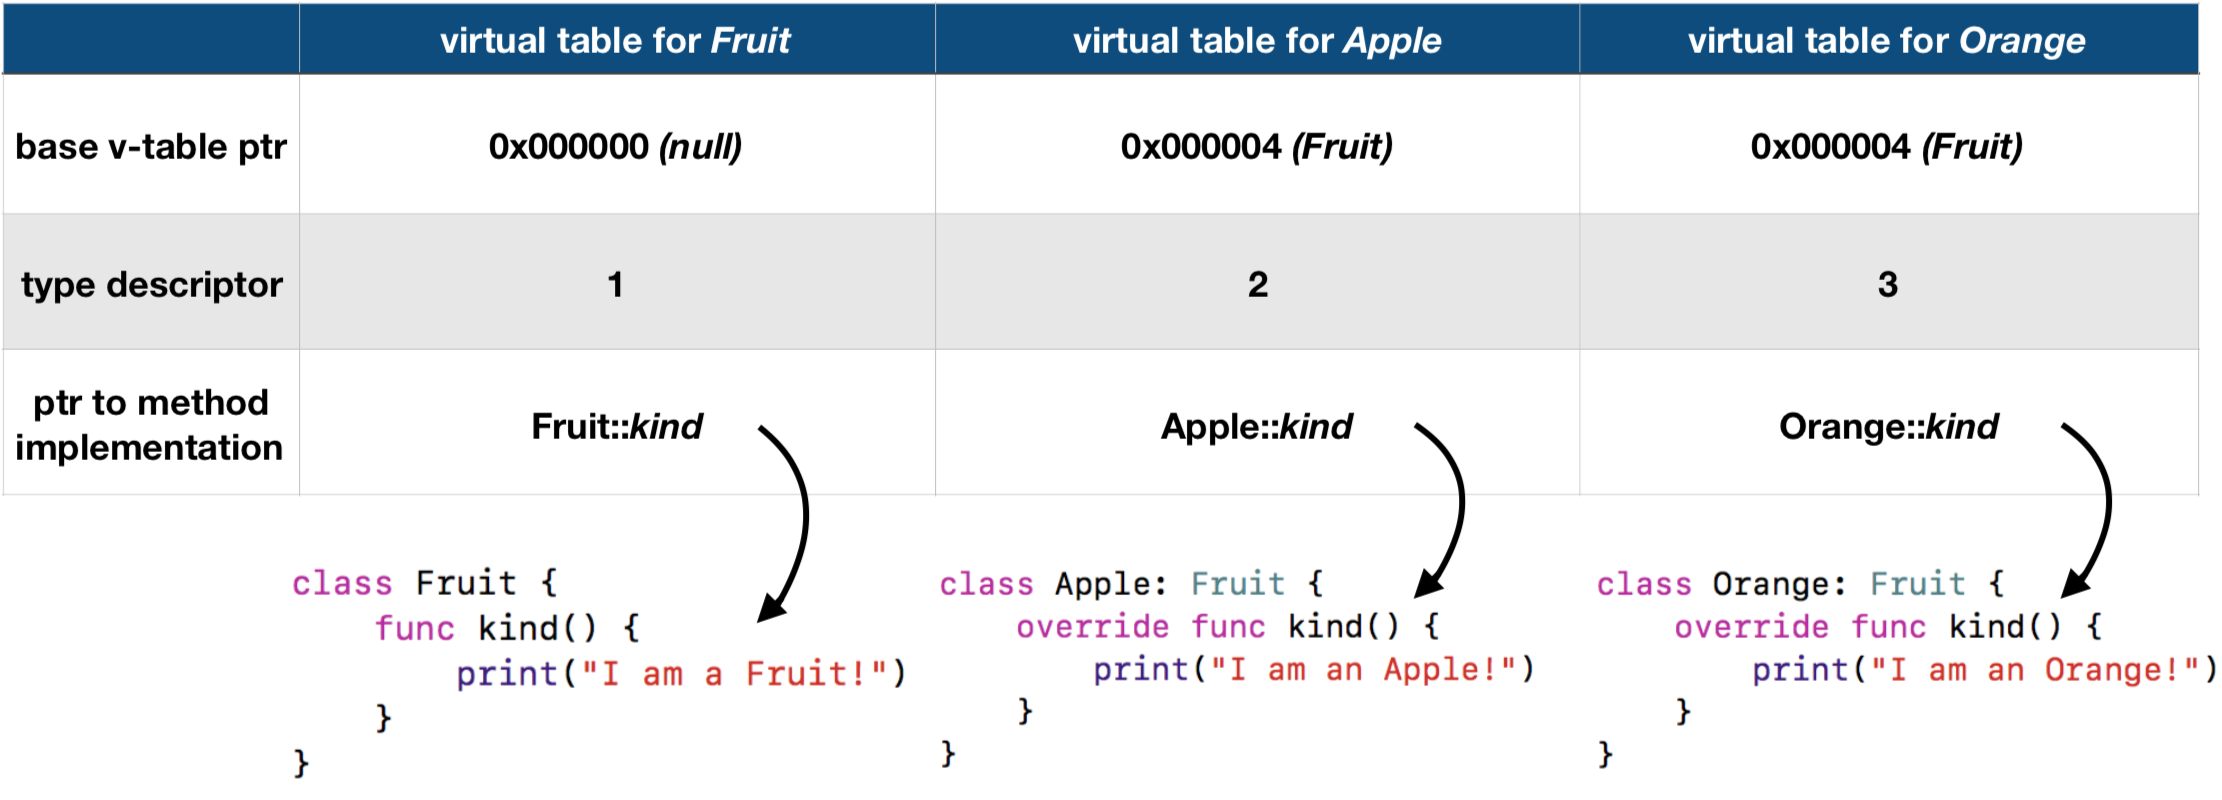
\includegraphics[width=1\textwidth]{resources/vtables.png}
	\end{center}
	\caption{Navidezne tabele za dane razrede iz ~\ref{virtualTableExamples}.}
	\label{vtables}
\end{figure}

\indent Vsak objekt v pomnilniku, poleg svojih atributov, hrani še kazalec na lastno virtualno tabelo.

\subsection{Realizacija}

Problem rešimo tako, da kazalec na metodo shranimo v virtualno tabelo na tisti indeks, na katerem je metoda definirana v razredu. Prevajalnik za klic funkcije zgenerira vmesno kodo, ki izračuna naslov metode z naslednjo enačbo:

\[ address(method_i) = adress(vtable) + (i * sizeof(void*) + 8) \]

kjer je \[address(vtable)\] lokacija tabele v pomnilniku, \[i * sizeof(void*) + 8\] indeks pomnožen z velikostjo kazalca (običajno 4 byti) plus odmik od začetka tabele zaradi prej opisanih dodatnih podatkov v tabeli in \[address(method_i)\] naslov metode na indeksu i.

\section{Vmesniki}

Vmesnik je abstraken opis akcij, ki jih lahko izvede objekt. Vmesnik je abstraktna podatkovna struktura, zato ne moremo kreirati instance neposredno, lahko pa spremeljivki priredimo instanco razreda, če razred implementira vmesnik. Vse metode so klicane dinamično, po postoku opisanem v razdelku \ref{dynamicDispatch}. \\
\indent Definirajmo preprost vmesnik ter ga implementirajmo v dveh razredih:

\begin{lstlisting}[caption={}, label={lst:interfaces}, captionpos=b]
	interface I {
	    func foo()
	}
	class A: I {
	    func foo() {
	        print("A's implementation of foo")
	    }
	}
	class B: I {
	    func foo() {
	        print("B's implementation of foo")
	    }
	}
	var x: I
	x = A()
	x.foo() # 'A's implementation of foo'
	x = B()
	x.foo() # 'B's implementation of foo'
\end{lstlisting}

\section{Abstraktni razredi}

Programski jezik Atheris dopušča zmožnost deklariranja abstraktnih razredov z uporabo rezervirane besede {\ttfamily abstract}. Značilnost abstraktnih razredov je to, da ne moremo kreirati njihovih instanc neposredno. Abstraktni razredi s tem dopuščajo možnost definiranja abstraktnih metod, ki jih mora vsak dedujoči se neabstraktni razred implementirati. V tem pogledu so si abstraktni razredi in vmesniki zelo podobni. Abstraktne metode definiramo tako kot razrede z uporabo ključne besede {\ttfamily abstract}. \\
\indent Program \ref{lst:abstractClassesEx} definira abstrakten razred \textit{Shape}, ki vsebuje abstraktno metodo za izračun površine lika (vsak lik izračuna lastno površino na drugačen način). Razreda \textit{Square} in \textit{Rect} dedujeta od abstraktnega razreda ter implementirata abstraktno metodo \textit{area}.

\begin{lstlisting}[caption={Primer uporabe abstraktnih razredov.}, captionpos=b, label={lst:abstractClassesEx}]
	abstract class Shape {
	    var len: Int
	    abstract func area() Int
	}
	class Square: Shape {
	    init(_ len: Int) {
	        self.len = len
	    }
	    func area() Int {
	        return self.len * self.len
	    }
	}
	class Rect: Shape {
	    var height: Int
	    init(width: Int, height: Int) {
	        self.len = width
	        self.height = height
	    }
	    func area() Int {
	        return self.len * self.height
	    }
	}
	
	var shape: Shape
	shape = Square(10)
	print(shape.area()) # '100'
	shape = Rect(width: 5, height: 10)
	print(shape.area())  # '50'
\end{lstlisting}

Naloga prevajalnika je, da zagotovi, da so v razredu implementirane vse abstraktne metode, ki so definirane v hiearhiji razredov. Če ne želimo implementirati vseh metod abstraktnega razreda, mora biti razred označen kot abstrakten. \\
\indent Definirajmo abstraktni podatkovni strukturi seznam in sklad, ki definirata ustrezne abstraktne operacije:

\begin{lstlisting}[caption={}, captionpos=b]
	abstract class AbstractList {
	    private var storage: [Int]
	    abstract func append(_ val: Int)
	    abstract func remove(at index: Int)
	}
	
	abstract class AbstractStack: AbstractList {
	    abstract func push()
	    abstract func pop()
	}
\end{lstlisting}

Razred, ki želi dedovati od \textit{AbstractStack}, mora poleg metod \textit{push} in \textit{pop} implementirati tudi obe metodi v \textit{AbstractList} razredu:

\begin{lstlisting}[caption={}, captionpos=b]
	class Stack: AbstractStack {
	    func append(_ val: Int) {}
	    func remove(at index: Int) {}
	    func push() {}
	    func pop() {}
	}
\end{lstlisting}

\section{Operator {\ttfamily is}}

Operator {\ttfamily is} (v Javi {\ttfamily instanceof}) je operator, ki v času izvajanja programa preveri, ali je objekt instanca danega razreda. To naredi z uporabo virtualne tabele. Kot je bilo omenjeno, vsaka tabela vsebuje unikatni deskriptor njenega razreda. Preko deskriptorja lahko preverimo, ali se dva podatkovna tipa ujemata. Ker je lahko razredna hiearhija obsežna, je potrebno preverjanje izvesti rekurzivno po celotni hiearhiji. \\
\indent Delovanje operatorja {\ttfamily is} je razvidno v programu \ref{lst:operatorIs}.

\begin{lstlisting}[caption={Uporaba operatorja {\ttfamily is}.}, captionpos=b, label={lst:operatorIs}]
	class A {}
	class B: A {}
	class C: A {}
	
	var object: A = B() # spremenljivki tipa 'A' priredimo objekt tipa 'B'
	print(object is A) # 'true'
	print(object is B) # 'true'
	print(object is C) # 'false'
\end{lstlisting}

\section{Pretvarjanje tipov - operator {\ttfamily as}}

Mehanizem dinamičnega pretvarjanja iz enega tipa v drugega (angl. \textit{type casting}) deluje po zelo podobnem principu kot {\ttfamily as} operator. Razlikujeta se predvsem v njunem rezultatu. Rezultat {\ttfamily is} operatorja je {\ttfamily true} ali {\ttfamily false}, za razliko od operatorja {\ttfamily as}, pri katerem je rezultat bodisi objekt pretvorjen v želen tip pri uspešni pretvorbi, bodisi {\ttfamily null} pri neuspešni. Tako pretvarjanje imenujemo varno pretvarjanje (angl. \textit{safe casting}), saj program nadaljuje z izvajanjem tudi če pretvorba ni uspešna.
\\\indent Delovanje operatorja {\ttfamily as} je razvidno v programu \ref{lst:operatorAs}.
\begin{lstlisting}[caption={Uporaba operatorja {\ttfamily as}.}, captionpos=b, label={lst:operatorAs}]
	class A {}
	class B: A {}
	let object: A = B()
	let casted = object as B
	if casted == nil {
	    print("cast failed")
	}
	else {
	    print("cast succeeded") # izvede se 'else' blok
	}
\end{lstlisting}

\section{Razširitve}

Razširitev (angl. \textit{extension}) je mehanizem, ki omogoča dodajanje funkcionalnosti obstoječim razredom. Razred lahko razširimo z metodami, enumeracijami in razredi. 
\\\indent Definirajmo prazen razred ter ga razširimo z različnimi definicijami:

\begin{lstlisting}[caption={}, captionpos=b]
	class A {}
	extension A {
		func toString() {
			print("ext::toString()")
		}
		class B {
			let x = 10
		}
		enum C: String {
			case a
		}
	}
	A().toString()
	print(A.B().x)
	print(A.C.a.rawValue)
\end{lstlisting}

Tekom prvega sprehoda po AST v fazi razreševanja imen prevajalnik vstavi v razredni podatkovni tip vse nove definicije, ki se nahajajo v razširitvi. Če se bomo v nadaljevanju programa sklicevali na definicijo, ki je definirana v razširitvi, jo tako bo DOT operator brez težav našel v samem razredu. \\
\indent V primeru, da definicija z istim imenom že obstaja, prevajalnik javi napako:

\begin{lstlisting}[caption={}, captionpos=b]
	class A {
	    func f() {}
	}
	extension A {
	    func f() {} # napaka
	}
\end{lstlisting}

\subsection{Razširitev z vmesnikom}

Razredom lahko preko razširitev dodamo tudi implementacijo vmesnikov, čemur rečemo \textit{razširitev z vmesnikom} (angl. \textit{interface extension}).
\\\indent Definirajmo razred ter mu dodajmo implementacijo vmesnika preko razširitve:

\begin{lstlisting}[caption={}, captionpos=b]
	class Collection {}
	interface Iterable {
	    func next() Int
	}
	extension Collection: Iterable {
	    func next() Int {
	        return 10
	    }
	}
	let iterable = Collection()
	print(iterable.next())
\end{lstlisting}

\section{Avtomatično prepoznavanje tipov}

Avtomatično prepoznavanje tipov (angl. \textit{type inference}) je sposobnost prevajalnika, da samodejno prepozna podatkovni tip izraza na podlagi vrednosti, ki so v izrazu. To je posebej uporabno pri definicijah spremeljivk, ki jim pogosto nastavimo vrednost ob sami definiciji. \\
\indent V primeru, da definicija spremenljivke nima eksplicitno navedenega podatkovnega tipa, prevajalnik najprej izračuna podatkovni tip izraza na desni strani prirejevalnega operatorja ter ga nato dodeli definiciji, kot je razvidno iz programa \ref{lst:typeInferenceEx}.

\begin{lstlisting}[caption={Avtomatično prepoznavanje podatkovnih tipov.}, captionpos=b, label={lst:typeInferenceEx}]
	let meaningOfLife = 42
	# meaningOfLife je tipa Int
	let pi = 3.14159
	# pi je tipa Double
	let robot = "Mr. Robot"
	# robot je tipa String
\end{lstlisting}

Prepoznavanje tipov postane kompleksno pri tabelah, kadar njeni elementi niso istih tipov. Prevajalnik vedno poišče najmanjši možen tip, ki je skupen vsem elementom tabele. V primeru, da so v tabeli objekti, ki jim je skupen nadrazred {\ttfamily A}, bo tudi tabela tipa {\ttfamily A} (prikazano v programu \ref{lst:arrayCommon}). V primeru, da elementi nimajo nobenega skupnega tipa, prevajalnik tabeli dodeli poseben abstrakten tip {\ttfamily Any}, ki je definiran v standardni knjižnici (prikazano v programu \ref{lst:arrayNoCommon}).

\begin{lstlisting}[caption={Elementi tabele s skupnim nadrazredom.}, captionpos=b, label={lst:arrayCommon}]
	class A {}
	class B: A {}
	class C: A {}
	let array = [C(), B(), C(), C()] 
	# spremenljivka array je tipa ARR ( A )
\end{lstlisting}

\begin{lstlisting}[caption={Elementi tabele nimajo skupnega tipa.}, captionpos=b, label={lst:arrayNoCommon}]
	let array = [10, "string", A(), 3.14] 
	# spremenljivka array je tipa ARR ( Any )
\end{lstlisting}

\begin{lstlisting}[caption={Spremenljivkam tipa \textit{Any} lahko priredimo vrednost poljubnega tipa.}, captionpos=b, label={lst:allAny}]
	let a: Any = 10
	let b: Any = 'X'
	let c: Any = "String"
	let d: Any = [10, 20, 30]
	let e: Any = 3.14
\end{lstlisting}
%
{\ttfamily Any} je v programskem jeziku Atheris to, kar je v Javi {\ttfamily Object}, s to razliko, da je {\ttfamily Object} razred, {\ttfamily Any} pa vmesnik. Vsak podatkovni tip je implicitno tudi tip {\ttfamily Any}, kot to lahko vidimo v programu \ref{lst:allAny}.

\chapter{Meritve in testiranje}

Delovanje programskega jezika Atheris je testirano na znanih algoritmih – \textit{bubblesort}, \textit{quicksort} in \textit{fibonacci}. Testni primeri so izbrani tako, da preko njih preizkusimo delovanje čim več funkcionalnosti jezika. Kot zanimivost je izmerjena tudi hitrost izvajanja programov in primerjana z osnovnim jezikom. Za referenco je izmerjena tudi hitrost delovanja algoritmov v Pythonu.

%\newpage

\section{Meritve}

\subsection{Bubblesort}

Z bubblesort algoritmom preverimo:

\begin{itemize}
	\item dostopanje do pomnilnika (do elementov v tabeli na nekem indeksu),
	\item delovanje zank,
	\item klicanje funkcij, prenos parametrov.
\end{itemize}
Algoritem smo izvedli 100.000-krat na številih \textit{8, 0, 3, 9, 2, 14, 10, 27, 1, 5, 8, -1, 26} in pri tem merili čas izvajanja.

\begin{figure}[h]
	\centering
\begin{tikzpicture}
\begin{axis}[
symbolic x coords={PINS, Atheris, Python},
xtick=data,
bar width=40,
width=300,
ylabel={Čas (sekunde)},
xlabel={Programski jezik}]
]
\addplot[ybar,fill=blue] coordinates {
	(PINS,   29.802)
	(Atheris,  28.535)
	(Python,   2.017)
};
\end{axis}
\end{tikzpicture}
\caption{Bubblesort (sortiranje z navadnimi zamenjavami).}
\label{meritveBubbleSort}
\end{figure}

Rezultati niso presenetljivi, PINS in Atheris potrebujeta približno enako časa, medtem ko je Python (po pričakovanjih) bistveno hitrejši (rezultati so vidni na sliki \ref{meritveBubbleSort}).

\subsection{Quicksort}

Z uporabo quicksort algoritma poleg prej naštetih funkcionalnosti testiramo še delovanje rekurzije. Algoritem je izveden pod enakimi pogoji kot bubblesort. Rezultati meritve so vidni na sliki \ref{meritveQuickSort}. \\

\begin{figure}
	\centering
\begin{tikzpicture}
\begin{axis}[
symbolic x coords={PINS, Atheris, Python},
xtick=data,
bar width=40,
width=300,
ylabel={Čas (sekunde)},
xlabel={Programski jezik}]
]
\addplot[ybar,fill=blue] coordinates {
	(PINS,   34.600)
	(Atheris,  18.449)
	(Python,   1.507)
};
\end{axis}
\end{tikzpicture}
\caption{Quicksort.}
\label{meritveQuickSort}
\end{figure}

Dobljen rezultat je izjemno zanimiv, saj je Atheris bistveno hitrejši kot PINS. Rezultat je zanimiv predvsem zato, ker prevajalnik za Atheris ne vsebuje veliko optimizacij napram osnovnemu prevajalniku.  \\
\indent Po podrobni analizi se izkaže, da sta za razliko v hitrosti izvajanja algoritma kriva predvsem dva razloga:

\begin{itemize}
	\item Programski jezik PINS ne podpira izrazov za prenos toka (angl. \textit{control transfer}). Običajno sta to {\ttfamily break} in {\ttfamily continue}. Algoritem je zato potrebno implementirati z uporabo začasnih spremenljivk, zaradi česar se izvede občutno večje število ukazov prirejanja in primerjanja.
	
	\item Drug razlog za tako občutno razliko pa je to, da je klicanje funkcij v Atherisu nekoliko hitrejše napram PINSu. Izkaže se da quicksort algoritem izvede veliko večje število klicev funkcij napram bubblesortu, kar je smiselno, glede na to, da je algoritem rekurziven. \\
	\indent Klici funkcij so v Atherisu implementirani tako, da se koda funkcije pred začetkom izvajanja programa shrani v pomnilnik, do kode pa dostopamo preko labele. Interpreter vsebuje preslikavo iz labele na naslov kode funkcije v pomnilniku, kar nam omogoča izvedbo funkcije. V PINSu funkcij ne shranjujemo v pomnilnik, ampak do njih dostopamo preko dveh slovarjev, ki preslikata labelo funkcije v njen klicni zapis in njeno kodo.
\end{itemize}

\subsection{Izračun n-tega fibonaccijevega števila}

Zadnji testni algoritem je izračun n-tega fibonaccijevega števila z uporabo rekurzivne enačbe
$fib(n) = fib(n - 1) + fib(n - 2) ; fib(0) = 1; fib(1) = 1$. Računamo $fib(35)$. \\
\indent Rezultat je prikazan na sliki \ref{meritveFibonacci}.

\begin{figure}
	\centering
\begin{tikzpicture}
\begin{axis}[
symbolic x coords={PINS, Atheris, Python},
xtick=data,
bar width=40,
width=300,
ylabel={Čas (sekunde)},
xlabel={Programski jezik}]
]
\addplot[ybar,fill=blue] coordinates {
	(PINS,  34.874)
	(Atheris, 32.308)
	(Python, 3.019)
};
\end{axis}
\end{tikzpicture}
\caption{Izračun n-tega fibonaccijevega števila.}
\label{meritveFibonacci}
\end{figure}

\subsection{Quicksort s polimorfnimi operacijami}

V razdelku ~\ref{dynamicDispatch} je podrobneje opisano delovanje polimorfnih operacij, kot so dinamično klicanje funkcij, operator {\ttfamily is} ter pretvarjanje tipov (operator {\ttfamily as}). Naštete operacije omogočajo priročne funkcionalnosti, ki nam pri razvoju programske opreme pogosto pridejo prav. A pod določeno ceno, saj je izvedba teh operacij relativno počasna. \\
\indent Zanimalo nas je, kakšna je pravzaprav dejanska cena, ki jo moramo plačati za njihovo izvajanje. Pripravljen je primer, ki testira prav to.
Gre za implementacijo quicksort algoritma, ki se izvaja nad identičnimi vhodnimi podatki kot prejšnji primeri, s to razliko, da so števila ovita v objekte. Izvajanje primerjanja dveh objektov poteka z uporabo naštetih polimorfnih operacij. Rezultat meritve je viden na sliki \ref{meritvePoli}.

\begin{figure}[!b]
	\centering
	\begin{tikzpicture}
\begin{axis}[
symbolic x coords={PINS, Atheris, Atheris - razredi},
xtick=data,
bar width=40,
width=300,
ylabel={Čas (sekunde)},
xlabel={Programski jezik}]
]
\addplot[ybar,fill=blue] coordinates {
	(PINS,   34.600)
	(Atheris,  18.449)
	(Atheris - razredi,   42.874)
};
\end{axis}
\end{tikzpicture}
\caption{Quicksort s polimorfnimi operacijami.}
\label{meritvePoli}
\end{figure}

Po pričakovanjih se izkaže, da je izvajanje res občutno počasnejše; in sicer za skoraj 230 \%. 

\chapter{Sklepne ugotovitve}

V okviru diplomskega dela so predstavljeni programski jeziki in prevajalniki, sodobne prakse načrtovanja in implementacije prevajalnikov ter njihova zgradba. Podrobneje sta opisana programska jezika PINS in Atheris, poudarek je na slednjem, ki je nadgradnja prvega. Razširitve, ki jih prevajalnik za Atheris vsebuje napram prevajalniku za PINS, in njihova implementacija, so tekom naloge podrobneje opisane. \\
\indent Programski jezik Atheris omogoča uporabo objektno usmerjenih gradnikov, ki jih vidimo v sodobnih objektnih jezikih; to so enumeracije, terke, razredi in vmesniki. Atheris podpira tudi razširitve razredov, podobno kot Swift. \\
\indent Za diplomsko delo je bilo načrtovano kar nekaj funkcionalnosti, ki zaenkrat še niso implementirane. Med njih spadajo generični podatkovni tipi in generične funkcije, opcijski podatkovni tipi in funkcijske ovojnice. Njihova vgradnja bo prišla na vrsto v nadaljnem razvoju prevajalnika. \\
\indent  V razdelku ~\ref{semanSection} smo omenili, da lahko semantična analiza stori več, kot le razreši imena in podatkovne tipe. Prevajalnik za Atheris vsebuje še tretjo semantično fazo, ki se imenuje \textit{preverjanje inicializiranosti}. Naloga te faze je, da za vsako spremenljivko zagotovi, da ji je bila pred njeno uporabo nastavljena vrednost. Poleg tega prepreči, da bi lahko konstantam priredili vrednost več kot enkrat. Faza je trenutno še v povojih in zaenkrat ne deluje tako, kot bi si želeli, zato v diplomskem delu ni opisana. \\
\indent Tekom diplomskega dela se osredotočamo predvsem na \textit{front-end} del prevajalnika, kjer se izvede analiza izvorne kode in sinteza v vmesno. Preskočili smo celoten zaledni del prevajalnika (\textit{back-end}). Naloga zalednega dela je optimizacija vmesne in generiranje dejanske strojne kode za ciljno arhitekturo. V prihodnje je cilj vgradnja izjemno močnega zalednega sistema  v \textbf{LLVM} \cite{LLVM}, na katerem temeljijo tudi zelo zmogljivi C++, Objective-C in Swift prevajalniki. \\
\indent Namesto vgradnje LLVM bi bilo zanimivo tudi prevajanje v Javin \textit{bytecode}, saj bi s tem pridobili vse zelo napredne sposobnosti JVM-ja. Primer takega jezika je Kotlin, ki se je izkazal kot zelo dober programski jezik, in je celo nadomestil Javo na področju razvoju programske opreme za Android platformo.


\chapter{Priloge} 

\section{Atheris}

\subsection{Bubblesort}

\begin{lstlisting}
func bubbleSort(_ list: [Int], size: Int) Int {
    var i = 0
    while i < size {
        var j = 0
        while j < size {
            if list[i] < list[j] {
                let tmp = list[i]
                list[i] = list[j]
                list[j] = tmp
            }
            j = j + 1
        }
        i = i + 1
    }
}

var list = [ 8, 0, 3, 9, 2, 14, 10, 27, 1, 5, 8, -1, 26 ]
var i = 0
while i < 100000 {
    bubbleSort(list, size: list.count)
    list[0] = 8
    list[1] = 0
    list[2] = 3
    list[3] = 9
    list[4] = 2
    list[5] = 14
    list[6] = 10
    list[7] = 27
    list[8] = 1
    list[9] = 5
    list[10] = 8
    list[11] = -1
    list[12] = 26
    i = i + 1
}
\end{lstlisting}

\subsection{Quicksort}

\begin{lstlisting}
func quickSort(_ list: [Int], low: Int, high: Int) {
    func partition(_ list: [Int], low: Int, high: Int) Int {
        let pivot = list[low]
        var i = low - 1
        var j = high + 1

        while true {
            while true {
                j = j - 1
                if list[j] <= pivot {
                    break
                }
            }

            while true {
                i = i + 1
                if list[i] >= pivot {
                    break
                }
            }

            if i < j {
                let tmp = list[i]
                list[i] = list[j]
                list[j] = tmp
            }
            else {
                return j
            }
        }
    }

    if low < high {
        let p = partition(list, low: low, high: high)
        quickSort(list, low: low, high: p)
        quickSort(list, low: p + 1, high: high)
    }
}

var list = [ 8, 0, 3, 9, 2, 14, 10, 27, 1, 5, 8, -1, 26 ]
var i = 0
while i < 100000 {
    quickSort(list, low: 0, high: list.count - 1)
    list[0] = 8
    list[1] = 0
    list[2] = 3
    list[3] = 9
    list[4] = 2
    list[5] = 14
    list[6] = 10
    list[7] = 27
    list[8] = 1
    list[9] = 5
    list[10] = 8
    list[11] = -1
    list[12] = 26
    i = i + 1
}
\end{lstlisting}

\subsection{Fibonacci}

\begin{lstlisting}
func fib(_ n: Int) Int {
    if n < 2 {
        return 1
    }
    else {
        return fib(n - 1) + fib(n - 2)
    }
}
fib(35)
\end{lstlisting}

\subsection{Quicksort nad objekti}

\begin{lstlisting}
class Comparable {
    func compare(with object: Any) Int {
        if object is Comparable {
            let comparable = object as Comparable
            return self.value() - comparable.value()
        }
        else {
            return 0
        }
    }

    func value() Int {
        return 0
    }

    func toString() {
    }
}

class Integer: Comparable {
    var val: Int

    init(_ val: Int) {
        self.val = val
    }

    override func value() Int {
        return self.val
    }

    override func toString() {
        print(self.val)
    }
}

class Decimal: Comparable {
    var val: Int

    init(_ val: Int) {
        self.val = val
    }

    override func value() Int {
        return self.val
    }

    override func toString() {
        print(self.val)
    }
}

func partition(_ list: [Comparable], low: Int, high: Int) Int {
    let pivot = list[low]
    var i = low - 1
    var j = high + 1

    while true {
        while true {
            j = j - 1
            let el = list[j]
            if el.compare(with: pivot) <= 0 {
                break
            }
        }

        while true {
            i = i + 1
            let el = list[i]
            if el.compare(with: pivot) >= 0 {
                break
            }
        }

        if i < j {
            let tmp = list[i]
            list[i] = list[j]
            list[j] = tmp
        }
        else {
            return j
        }
    }
}

func quicksort(_ list: [Comparable], low: Int, high: Int) {
    if low < high {
        let p = partition(list, low: low, high: high)
        quicksort(list, low: low, high: p)
        quicksort(list, low: p + 1, high: high)
    }
}

var list = [ Integer(8), Decimal(0), Integer(3), Integer(9), Decimal(14), Decimal(10), Integer(27), Decimal(1), Decimal(5), Integer(8), Decimal(-1), Decimal(26) ]

var i = 0
while i < 100000 {
    quicksort(list, low: 0, high: list.count - 1)
    i = i + 1
}
\end{lstlisting}

\section{PINS}\label{primeriPins}

\subsection{Bubblesort}

\begin{lstlisting}
fun bubble(tab:arr[13] integer) : integer = (
    {for i = 0, 13, 1 :
        {for j = 0, 13, 1:
            {if tab[j] > tab[i] then 
                (
                {tmp = tab[j]},
                {tab[j] = tab[i]},
                {tab[i] = tmp}, 0
                ) 
                { where var tmp : integer} 
            }
        }
    },
    1
) { where var i : integer; var j : integer };

var tab: arr[13] integer;
var count: integer;

fun main(i:integer) : integer = (
    {while count < 100000:
        (
        {tab[0] = 8},
        {tab[1] = 0},
        {tab[2] = 3},
        {tab[3] = 9},
        {tab[4] = 2},
        {tab[5] = 14},
        {tab[6] = 10},
        {tab[7] = 27},
        {tab[8] = 1},
        {tab[9] = 5},
        {tab[10] = 8},
        {tab[11] = -1},
        {tab[12] = 26},
        bubble(tab),
        {count = count + 1}
        )
    },
    0
)
\end{lstlisting}


\subsection{Quicksort}

\begin{lstlisting}
fun partition(tab: arr[13] integer, low: integer, high: integer) : integer = (
    {pivot = tab[low]},
    {i = low - 1},
    {j = high + 1},
    {loop = true},
    {while loop == true:
        (
        {p = true},
        {while p == true:
            (
            {j = j - 1},
            {if tab[j] <= pivot then
                {p = false}
            }
            )
        },
        {p = true},
        {while p == true:
            (
            {i = i + 1},
            {if tab[i] >= pivot then
               {p = false}
            }
            )
        },
        {if i < j then
            (
            {tmp = tab[j]},
            {tab[j] = tab[i]},
            {tab[i] = tmp},0
            )
        { where var tmp : integer}
        else ({loop = false})
        }
        )
    },
    j
) { where var pivot: integer; var i: integer; var j: integer; var p: logical; var loop: logical };

fun quickSort(tab: arr[13] integer, low: integer, high: integer) : integer = (
    {if low < high then
        (
        {p = partition(tab, low, high)},
        quickSort(tab, low, p),
        quickSort(tab, p + 1, high)
        )
    },
    0
) { where var p: integer }

var tab: arr[13] integer;
var count: integer;

fun main(i:integer) : integer = (
    {while count < 100000:
        (
        {tab[0] = 8},
        {tab[1] = 0},
        {tab[2] = 3},
        {tab[3] = 9},
        {tab[4] = 2},
        {tab[5] = 14},
        {tab[6] = 10},
        {tab[7] = 27},
        {tab[8] = 1},
        {tab[9] = 5},
        {tab[10] = 8},
        {tab[11] = -1},
        {tab[12] = 26},
        quickSort(tab, 0, tab.length - 1),
        {count = count + 1}
        )
    },
    0
)
\end{lstlisting}


\subsection{Fibonacci}

\begin{lstlisting}
fun fib(x : integer) : integer = (
    { if x < 2 then
        ({rez = 1})
    else 
        ({rez = fib(x - 1) + fib(x - 2)})
    },
    rez
) {where var rez : integer};

fun main(i:integer) : integer = (
    {i = fib(35)},
    0
)
\end{lstlisting}

\section{Python}

\subsection{Bubblesort}

\begin{lstlisting}
def bubble(list):
    for i in range(len(list)):
        for j in range(len(list)):
            if list[i] < list[j]:
                tmp = list[i]
                list[i] = list[j]
                list[j] = tmp

startTime = time.time()

list = [ 8, 0, 3, 9, 2, 14, 10, 27, 1, 5, 8, -1, 26 ]
for i in range(100000):
    bubble(list)
    list = [8, 0, 3, 9, 2, 14, 10, 27, 1, 5, 8, -1, 26]
print(time.time() - startTime)
\end{lstlisting}


\subsection{Quicksort}

\begin{lstlisting}
import time

def partition(list, low, high):
    pivot = list[low]
    i = low - 1
    j = high + 1

    while True:
        while True:
            j = j - 1
            if list[j] <= pivot:
                break

        while True:
            i = i + 1
            if list[i] >= pivot:
                break

        if i < j:
            tmp = list[i]
            list[i] = list[j]
            list[j] = tmp
        else:
            return j

def quickSort(list, low, high):
    if low < high:
        p = partition(list, low, high)
        quickSort(list, low, p)
        quickSort(list, p + 1, high)

startTime = time.time()

list = [ 8, 0, 3, 9, 2, 14, 10, 27, 1, 5, 8, -1, 26 ]
for i in range(100000):
    quickSort(list, 0, len(list) - 1)
    list = [8, 0, 3, 9, 2, 14, 10, 27, 1, 5, 8, -1, 26]
print(time.time() - startTime)
\end{lstlisting}

\subsection{Fibonacci}

\begin{lstlisting}
import time

def fib(n):
    if n < 2:
        return 1
    return fib(n - 1) + fib(n - 2)

startTime = time.time()
fib(35)
print(time.time() - startTime)
\end{lstlisting}

\newpage %dodaj po potrebi, da bo številka strani za Literaturo v Kazalu pravilna!

\clearpage
\addcontentsline{toc}{chapter}{Literatura}
\bibliographystyle{plain}
\bibliography{literatura}

\end{document}

